% Copyright (C) 2013 Columbia University in the City of New York and others.
%
% Please see the AUTHORS file in the main source directory for a full list
% of contributors.
%
% This file is part of TerraFERMA.
%
% TerraFERMA is free software: you can redistribute it and/or modify
% it under the terms of the GNU Lesser General Public License as published by
% the Free Software Foundation, either version 3 of the License, or
% (at your option) any later version.
%
% TerraFERMA is distributed in the hope that it will be useful,
% but WITHOUT ANY WARRANTY; without even the implied warranty of
% MERCHANTABILITY or FITNESS FOR A PARTICULAR PURPOSE. See the
% GNU Lesser General Public License for more details.
%
% You should have received a copy of the GNU Lesser General Public License
% along with TerraFERMA. If not, see <http://www.gnu.org/licenses/>.

\documentclass[10pt,twoside,openright]{memoir}
% Copyright (C) 2013 Columbia University in the City of New York and others.
%
% Please see the AUTHORS file in the main source directory for a full list
% of contributors.
%
% This file is part of TerraFERMA.
%
% TerraFERMA is free software: you can redistribute it and/or modify
% it under the terms of the GNU Lesser General Public License as published by
% the Free Software Foundation, either version 3 of the License, or
% (at your option) any later version.
%
% TerraFERMA is distributed in the hope that it will be useful,
% but WITHOUT ANY WARRANTY; without even the implied warranty of
% MERCHANTABILITY or FITNESS FOR A PARTICULAR PURPOSE. See the
% GNU Lesser General Public License for more details.
%
% You should have received a copy of the GNU Lesser General Public License
% along with TerraFERMA. If not, see <http://www.gnu.org/licenses/>.

\usepackage[english]{babel}
%\usepackage{tgtermes}
\usepackage[colorlinks=true]{hyperref}

\usepackage{mathpazo}
\usepackage[protrusion=true,expansion=true]{microtype}
\usepackage{lettrine}
\usepackage{graphicx}
\usepackage{amsfonts,amsmath,amssymb,amsthm,amsbsy,amssymb,bm}
\usepackage{xcolor}
\usepackage{enumitem}

\usepackage[square,sort,comma,numbers]{natbib}
\usepackage{rotating}
\setlength\fboxrule{0.0pt}
\setlength\fboxsep{0pt}

% Units
\usepackage{units}

\newcommand{\m}[1][]{\unit[#1]{m}}
\newcommand{\mm}[1][]{\unit[#1]{mm}}
\newcommand{\km}[1][]{\unit[#1]{km}}
\newcommand{\s}[1][]{\unit[#1]{s}}
\newcommand{\hrs}[1][]{\unit[#1]{hrs}}
\newcommand{\invs}[1][]{\unit[#1]{s}\ensuremath{^{-1}}}
\newcommand{\ms}[1][]{\unit[#1]{m\ensuremath{\,}s\ensuremath{^{-1}}}}
\newcommand{\mss}[1][]{\unit[#1]{m\ensuremath{\,}s\ensuremath{^{-2}}}}
\newcommand{\J}[1][]{\unit[#1]{J}}
\newcommand{\K}[1][]{\unit[#1]{K}}
\newcommand{\W}[1][]{\unit[#1]{W}}
\newcommand{\PSU}[1][]{\unit[#1]{PSU}}
\newcommand{\Pa}[1][]{\unit[#1]{Pa}}
\newcommand{\kg}[1][]{\unit[#1]{kg}}
\newcommand{\rads}[1][]{\unit[#1]{rad\ensuremath{\,}s\ensuremath{^{-1}}}}
\newcommand{\kgmm}[1][]{\unit[#1]{kg\ensuremath{\,}m\ensuremath{^{-2}}}}
\newcommand{\kgmmm}[1][]{\unit[#1]{kg\ensuremath{\,}m\ensuremath{^{-3}}}}
\newcommand{\Nmm}[1][]{\unit[#1]{N\ensuremath{\,}m\ensuremath{^{-2}}}}
\newcommand\Celsius{\ensuremath{^\circ}\unit{C}}


\usepackage[final]{listings}
\lstloadlanguages{[LaTeX]TeX,Python,bash,[gnu]Make,XML}

\lstset{basicstyle=\footnotesize\ttfamily,
  emph=anyfield,
  emphstyle=\textit,
  morekeywords={pure},
  escapeinside=`'
}

\lstdefinestyle{Bash}{
  language=bash,
  basicstyle=\small\sffamily,
  frame=tb,
  columns=fullflexible,
  backgroundcolor=\color{yellow!20},
  linewidth=0.9\linewidth,
  xleftmargin=0.1\linewidth
}

\lstdefinestyle{UFL}{
  language=Python,
  basicstyle=\small\ttfamily,
  numbers=left,
  numberstyle=\tiny,
  numbersep=3pt,
  frame=tb,
  columns=fullflexible,
  backgroundcolor=\color{yellow!20},
  linewidth=0.9\linewidth,
  xleftmargin=0.1\linewidth
}
\lstdefinestyle{python}{
  language=Python,
  basicstyle=\small\sffamily,
  numbers=left,
  numberstyle=\tiny,
  numbersep=3pt,
  frame=tb,
  columns=fullflexible,
  backgroundcolor=\color{yellow!20},
  linewidth=0.9\linewidth,
  xleftmargin=0.1\linewidth
}

%%%%%%%%%%%%tikz stuff
\usepackage{tikz}
\tikzstyle{every picture}+=[remember picture]

\tikzset{onslide/.code args={<#1>#2}{%
  \only<#1>{\pgfkeysalso{#2}} % \pgfkeysalso doesn't change the path
}}
\tikzstyle{highlightred}=[shape=rectangle, rounded corners, fill=red!50]
\tikzstyle{highlightgreen}=[shape=rectangle, rounded corners, fill=green!50]

\usetikzlibrary{fit, positioning, trees}
\usetikzlibrary{decorations.markings}
\usetikzlibrary{arrows,shapes}
\tikzstyle arrowstyle=[scale=1]
\tikzset{%
  highlight/.style={rectangle,rounded corners,fill opacity=0.5,inner sep=0pt}
}
\newcommand{\tikzmark}[2]{\tikz[overlay,remember picture,baseline=(#1.base)] \node (#1) {#2};}
%
\newcommand{\tikzhighlight}[4]{%
    \tikz[overlay,remember picture]{
    \node[highlight,fill=#4,fit=(#2.north west) (#3.south east)] (#1) {};}
}

\newcommand{\tikztermhighlight}[3]{\tikz[baseline=(#2.base)] \node[onslide=<#1>{highlightred}] (#2) {#3};}
\newcommand{\tikztermhighlightgreen}[3]{\tikz[baseline=(#2.base)] \node[onslide=<#1>{highlightgreen}] (#2) {#3};}

\tikzset{hide on/.code={\only<#1>{\pgfkeysalso{opacity=0}}}}

\tikzstyle directed=[postaction={decorate,decoration={markings,
    mark=at position 1.0 with {\arrow[arrowstyle]{stealth}}}}]
\tikzstyle reverse directed=[postaction={decorate,decoration={markings,
    mark=at position .65 with
    {\arrowreversed[arrowstyle]{stealth};}}}]
%%%%%%%%%%%%%%%%%%%%%%%%%%%%%
\usepackage{macros}
\addtolength{\textwidth}{2cm}
\addtolength{\foremargin}{-2cm}
\checkandfixthelayout

% See the ``Memoir customise'' template for some common customisations
% Don't forget to read the Memoir manual: memman.pdf

%% BEGIN TITLE

\makeatletter
\def\maketitle{%
  \null
  \thispagestyle{empty}%
  \vfill
  \begin{center}\leavevmode
    \normalfont
    {\LARGE\raggedleft \@author\par}%
    \hrulefill\par
    {\huge\raggedright \@title\par}%
    %\vskip 1cm
    \vfill
    {\Large \@date\par}%
  \end{center}%
  %\vfill
  \null
  \cleardoublepage
  }
\makeatother
\author{Cian Wilson and Marc Spiegelman }
\title{\TF{} Benchmarks}
\date{\today}


%%% HEADERS & FOOTERS
\pagestyle{ruled} % try also: empty , plain , headings , ruled , Ruled , companion

%%% CHAPTERS
\chapterstyle{demo} % try also: default , section , hangnum , companion , article, demo

%%% Change section number depth
\setsecnumdepth{subsection}
\setcounter{tocdepth}{2}

%%% clean up bib with Siam.bst \sc{} is not supported for some reason
\renewcommand{\sc}{}






%\includeonly{chapter1,chapter2,chapter3}
%\includeonly{chapter4}
%%% BEGIN DOCUMENT

\begin{document}
\pagestyle{headings}
\let\cleardoublepage\clearpage
\maketitle
\frontmatter

\null\vfill

\begin{flushleft}
\textit{A description of benchmarks for \TF}


\copyright{Copyright (C) 2013 Columbia University in the City of New York and others.}












\end{flushleft}
\let\cleardoublepage\clearpage

\newpage
\tableofcontents*
\mainmatter
\sloppy
% Copyright (C) 2013 Columbia University in the City of New York and others.
%
% Please see the AUTHORS file in the main source directory for a full list
% of contributors.
%
% This file is part of TerraFERMA.
%
% TerraFERMA is free software: you can redistribute it and/or modify
% it under the terms of the GNU Lesser General Public License as published by
% the Free Software Foundation, either version 3 of the License, or
% (at your option) any later version.
%
% TerraFERMA is distributed in the hope that it will be useful,
% but WITHOUT ANY WARRANTY; without even the implied warranty of
% MERCHANTABILITY or FITNESS FOR A PARTICULAR PURPOSE. See the
% GNU Lesser General Public License for more details.
%
% You should have received a copy of the GNU Lesser General Public License
% along with TerraFERMA. If not, see <http://www.gnu.org/licenses/>.

\chapter{Introduction} \label{sec:app}

In this supplemental material we provide the results of several well known benchmarks using \TF{}.  For each case we provide a brief description of the benchmark and the convergence results produced using \TF{} as compared to published solutions, where available.  When the non-dimensionalization used in the residual differs from that in the literature our results have been rescaled for comparison. Descriptions of each of the benchmark values listed in the tables can be found in the original papers.   Complete and reproducible \texttt{tfml} files and meshes for  the benchmarks can be found as a separate git repository at \url{bitbucket.org/tferma/benchmarks}.




% Copyright (C) 2013 Columbia University in the City of New York and others.
%
% Please see the AUTHORS file in the main source directory for a full list
% of contributors.
%
% This file is part of TerraFERMA.
%
% TerraFERMA is free software: you can redistribute it and/or modify
% it under the terms of the GNU Lesser General Public License as published by
% the Free Software Foundation, either version 3 of the License, or
% (at your option) any later version.
%
% TerraFERMA is distributed in the hope that it will be useful,
% but WITHOUT ANY WARRANTY; without even the implied warranty of
% MERCHANTABILITY or FITNESS FOR A PARTICULAR PURPOSE. See the
% GNU Lesser General Public License for more details.
%
% You should have received a copy of the GNU Lesser General Public License
% along with TerraFERMA. If not, see <http://www.gnu.org/licenses/>.

\chapter{Incompressible Two-Dimensional Convection: \citeauthor{BlankenbachGJI1989}} \label{sec:blankenbach}

\citet{BlankenbachGJI1989} described several benchmarks for
incompressible convection in a two-dimensional domain of unit height
and aspect ratio $l$.  The prognostic variables are velocity, $\vec{v}$,
pressure $p$, and temperature, $T$.

For the steady-state cases (1--2) boundary conditions for temperature are $T=0$ at the top surface, $z=1$, $T=1$ at the base, $z=0$,
with insulating (homogeneous Neumann, $\partial_x T = 0$) side-walls.  For velocity, free-slip boundary conditions are specified at
all boundaries.  Simulations are run at a variety of resolutions, all structured but with refinement at the boundaries, until a near
steady-state is attained where the variation in the fields is less than $10^{-9}$ in the infinity-norm between time-steps.

\paragraph{Case 1a--c}
Isoviscous steady-state cases are defined in a domain with aspect ratio, $l=1$,
with Rayleigh numbers $10^4$, $10^{5}$
and $10^{6}$ (Table \ref{tab:blankenbach1a-c})

\begin{table*}[th!]
\caption{Results from 2D, isoviscous square convection benchmark
  cases \citep{BlankenbachGJI1989}.}
\begin{center}
  \begin{tabular}{ll}
\fbox{\begin{minipage}[c]{0.025\textwidth}\begin{sideways}Case 1a: $\Ra=10^{4}$\end{sideways}\end{minipage}} 
&
\fbox{\begin{minipage}[c]{0.65\textwidth}\begin{tabular}{cccc}
     $N$ & $c\Delta t/\delta$  & $||\epsilon_{\phi}||$ & $\epsilon_{c}$  \\
32$\times$32 & 2.00 & 1.427786e-02 & 1.182138e-02  \\
32$\times$32 & 1.00 & 3.819159e-03 & 3.255477e-03  \\
32$\times$32 & 0.50 & 1.634865e-03 & 8.485232e-04  \\
32$\times$32 & 0.25 & 2.202831e-03 & 3.357135e-04  \\
64$\times$64 & 2.00 & 1.424202e-02 & 1.188175e-02  \\
64$\times$64 & 1.00 & 3.690917e-03 & 3.187174e-03  \\
64$\times$64 & 0.50 & 9.481209e-04 & 8.235713e-04  \\
64$\times$64 & 0.25 & 4.243532e-04 & 1.921914e-04  \\
128$\times$128 & 2.00 & 1.424087e-02 & 1.188190e-02  \\
128$\times$128 & 1.00 & 3.686779e-03 & 3.194658e-03  \\
128$\times$128 & 0.50 & 9.306871e-04 & 8.119311e-04  \\
128$\times$128 & 0.25 & 2.365556e-04 & 2.073026e-04  \\
\end{tabular}
\end{minipage}} \\
\\
\fbox{\begin{minipage}[c]{0.025\textwidth}\begin{sideways}Case 1b: $\Ra=10^{5}$\end{sideways}\end{minipage}} 
&
\fbox{\begin{minipage}[c]{0.65\textwidth}\begin{tabular}{cccc}
     $N$ & $c\Delta t/\delta$  & $||\epsilon_{\phi}||$ & $\epsilon_{c}$  \\
32$\times$32 & 2.00 & 1.427786e-02 & 1.182138e-02  \\
32$\times$32 & 1.00 & 3.819159e-03 & 3.255477e-03  \\
32$\times$32 & 0.50 & 1.634865e-03 & 8.485232e-04  \\
32$\times$32 & 0.25 & 2.202831e-03 & 3.357135e-04  \\
64$\times$64 & 2.00 & 1.424202e-02 & 1.188175e-02  \\
64$\times$64 & 1.00 & 3.690917e-03 & 3.187174e-03  \\
64$\times$64 & 0.50 & 9.481209e-04 & 8.235713e-04  \\
64$\times$64 & 0.25 & 4.243532e-04 & 1.921914e-04  \\
128$\times$128 & 2.00 & 1.424087e-02 & 1.188190e-02  \\
128$\times$128 & 1.00 & 3.686779e-03 & 3.194658e-03  \\
128$\times$128 & 0.50 & 9.306871e-04 & 8.119311e-04  \\
128$\times$128 & 0.25 & 2.365556e-04 & 2.073026e-04  \\
\end{tabular}
\end{minipage}} \\
\\
\fbox{\begin{minipage}[c]{0.025\textwidth}\begin{sideways}Case 1c: $\Ra=10^{6}$\end{sideways}\end{minipage}} 
&
\fbox{\begin{minipage}[c]{0.65\textwidth}\begin{tabular}{cccc}
     $N$ & $c\Delta t/\delta$  & $||\epsilon_{\phi}||$ & $\epsilon_{c}$  \\
32$\times$32 & 2.00 & 1.427786e-02 & 1.182138e-02  \\
32$\times$32 & 1.00 & 3.819159e-03 & 3.255477e-03  \\
32$\times$32 & 0.50 & 1.634865e-03 & 8.485232e-04  \\
32$\times$32 & 0.25 & 2.202831e-03 & 3.357135e-04  \\
64$\times$64 & 2.00 & 1.424202e-02 & 1.188175e-02  \\
64$\times$64 & 1.00 & 3.690917e-03 & 3.187174e-03  \\
64$\times$64 & 0.50 & 9.481209e-04 & 8.235713e-04  \\
64$\times$64 & 0.25 & 4.243532e-04 & 1.921914e-04  \\
128$\times$128 & 2.00 & 1.424087e-02 & 1.188190e-02  \\
128$\times$128 & 1.00 & 3.686779e-03 & 3.194658e-03  \\
128$\times$128 & 0.50 & 9.306871e-04 & 8.119311e-04  \\
128$\times$128 & 0.25 & 2.365556e-04 & 2.073026e-04  \\
\end{tabular}
\end{minipage}}
  \end{tabular}
\end{center}
  \label{tab:blankenbach1a-c}
\end{table*}

\paragraph{Case 2a-b}

Two variable viscosity steady-state cases were run. For case \textbf{2a},
viscosity is temperature dependent with 
\begin{equation}
 \mu = \exp\left(-bT_i\right)
\end{equation}
and $b=\ln(1000)$.
For case \textbf{2b} the viscosity is also depth-dependent according to the equation:
\begin{equation}
 \mu = \exp\left(-bT_i + c(1-z)\right)
\end{equation}
where $b=\ln(16384)$ and $c=\ln(64)$.
Convergence results are given in Table \ref{tab:blankenbach2a-b} for
$\Ra=10^4$, aspect ratio $l=1$.

\begin{table*}[th!]
\caption{Results from 2D, variable viscosity square convection benchmark
  cases $\Ra=10^{4}$ \citep{BlankenbachGJI1989}.}
\begin{center}
  \begin{tabular}{ll}
\fbox{\begin{minipage}[c]{0.025\textwidth}\begin{sideways}Case 2a: $\eta(T)$\end{sideways}\end{minipage}} 
&
\fbox{\begin{minipage}[c]{0.925\textwidth}\begin{tabular}{cccc}
     $N$ & $c\Delta t/\delta$  & $||\epsilon_{\phi}||$ & $\epsilon_{c}$  \\
32$\times$32 & 2.00 & 1.427786e-02 & 1.182138e-02  \\
32$\times$32 & 1.00 & 3.819159e-03 & 3.255477e-03  \\
32$\times$32 & 0.50 & 1.634865e-03 & 8.485232e-04  \\
32$\times$32 & 0.25 & 2.202831e-03 & 3.357135e-04  \\
64$\times$64 & 2.00 & 1.424202e-02 & 1.188175e-02  \\
64$\times$64 & 1.00 & 3.690917e-03 & 3.187174e-03  \\
64$\times$64 & 0.50 & 9.481209e-04 & 8.235713e-04  \\
64$\times$64 & 0.25 & 4.243532e-04 & 1.921914e-04  \\
128$\times$128 & 2.00 & 1.424087e-02 & 1.188190e-02  \\
128$\times$128 & 1.00 & 3.686779e-03 & 3.194658e-03  \\
128$\times$128 & 0.50 & 9.306871e-04 & 8.119311e-04  \\
128$\times$128 & 0.25 & 2.365556e-04 & 2.073026e-04  \\
\end{tabular}
\end{minipage}} \\
\\
\fbox{\begin{minipage}[c]{0.025\textwidth}\begin{sideways}Case 2b: $\eta(T,z)$\end{sideways}\end{minipage}} 
&
\fbox{\begin{minipage}[c]{0.925\textwidth}\begin{tabular}{cccc}
     $N$ & $c\Delta t/\delta$  & $||\epsilon_{\phi}||$ & $\epsilon_{c}$  \\
32$\times$32 & 2.00 & 1.427786e-02 & 1.182138e-02  \\
32$\times$32 & 1.00 & 3.819159e-03 & 3.255477e-03  \\
32$\times$32 & 0.50 & 1.634865e-03 & 8.485232e-04  \\
32$\times$32 & 0.25 & 2.202831e-03 & 3.357135e-04  \\
64$\times$64 & 2.00 & 1.424202e-02 & 1.188175e-02  \\
64$\times$64 & 1.00 & 3.690917e-03 & 3.187174e-03  \\
64$\times$64 & 0.50 & 9.481209e-04 & 8.235713e-04  \\
64$\times$64 & 0.25 & 4.243532e-04 & 1.921914e-04  \\
128$\times$128 & 2.00 & 1.424087e-02 & 1.188190e-02  \\
128$\times$128 & 1.00 & 3.686779e-03 & 3.194658e-03  \\
128$\times$128 & 0.50 & 9.306871e-04 & 8.119311e-04  \\
128$\times$128 & 0.25 & 2.365556e-04 & 2.073026e-04  \\
\end{tabular}
\end{minipage}}
  \end{tabular}
\end{center}
  \label{tab:blankenbach2a-b}
\end{table*}
 


% Copyright (C) 2013 Columbia University in the City of New York and others.
%
% Please see the AUTHORS file in the main source directory for a full list
% of contributors.
%
% This file is part of TerraFERMA.
%
% TerraFERMA is free software: you can redistribute it and/or modify
% it under the terms of the GNU Lesser General Public License as published by
% the Free Software Foundation, either version 3 of the License, or
% (at your option) any later version.
%
% TerraFERMA is distributed in the hope that it will be useful,
% but WITHOUT ANY WARRANTY; without even the implied warranty of
% MERCHANTABILITY or FITNESS FOR A PARTICULAR PURPOSE. See the
% GNU Lesser General Public License for more details.
%
% You should have received a copy of the GNU Lesser General Public License
% along with TerraFERMA. If not, see <http://www.gnu.org/licenses/>.

\chapter{Incompressible Three-Dimensional Convection: \citeauthor{Busse1993}} \label{sec:busse}

\citet{Busse1993} described several benchmarks for
incompressible convection in a three-dimensional domain of unit height
and aspect ratio in the horizontal dimensions of $a$ and $b$.  The prognostic variables are velocity, $\vec{v}$,
pressure $p$, and temperature, $T$.

For the steady-state cases considered (1a and 2) boundary conditions for temperature are $T=0$ at the top surface, $z=1$, $T=1$ at the base, $z=0$,
with insulating (homogeneous Neumann, $\nabla T\cdot\vec{n} = 0$) side-walls.  For velocity the top surface and base have no-slip
boundary conditions applied while all vertical sides impose free-slip conditions.
Simulations are run using full time-dependence on a coarse mesh until the solution reaches an approximate steady state.  This
solution is then interpolated to a variety of higher resolutions and used as an initial guess to solve the true steady state
problem.

\paragraph{Case 1a}
Isoviscous steady-state cases are defined in a domain with aspect ratio, $a=1.0079$, $b=0.6283$,
with a Rayleigh number of $3\times10^4$ (Table \ref{tab:busse1a}).

\begin{table*}[th!]
\caption{Results from 3D, isoviscous convection benchmark case 1a \citep{Busse1993}.}
\begin{center}
\begin{tabular}{cccc}
     $N$ & $c\Delta t/\delta$  & $||\epsilon_{\phi}||$ & $\epsilon_{c}$  \\
32$\times$32 & 2.00 & 1.427786e-02 & 1.182138e-02  \\
32$\times$32 & 1.00 & 3.819159e-03 & 3.255477e-03  \\
32$\times$32 & 0.50 & 1.634865e-03 & 8.485232e-04  \\
32$\times$32 & 0.25 & 2.202831e-03 & 3.357135e-04  \\
64$\times$64 & 2.00 & 1.424202e-02 & 1.188175e-02  \\
64$\times$64 & 1.00 & 3.690917e-03 & 3.187174e-03  \\
64$\times$64 & 0.50 & 9.481209e-04 & 8.235713e-04  \\
64$\times$64 & 0.25 & 4.243532e-04 & 1.921914e-04  \\
128$\times$128 & 2.00 & 1.424087e-02 & 1.188190e-02  \\
128$\times$128 & 1.00 & 3.686779e-03 & 3.194658e-03  \\
128$\times$128 & 0.50 & 9.306871e-04 & 8.119311e-04  \\
128$\times$128 & 0.25 & 2.365556e-04 & 2.073026e-04  \\
\end{tabular}

\end{center}
  \label{tab:busse1a}
\end{table*}
%
%\paragraph{Case 2}
%
%In the variable viscosity case, the
%viscosity is temperature dependent with 
%\begin{equation}
% \mu = \exp\left[Q/(T+G) - Q/(0.5+G)\right]
%\end{equation}
%where
%\begin{gather}
%Q = [255/\log{r}] - 0.25\log{r} \\
%G = [15/\log{r}] - 0.5
%\end{gather}
%with $r = \eta(T=0)/\eta(T=1) = 20$.
%Convergence results are given in Table \ref{tab:busse2} for
%$\Ra=2\times10^4$, aspect ratio $a=b=1$.
%
%\begin{table*}[th!]
%\caption{Results from 3D, variable viscosity convection benchmark case 2 \citep{Busse1993}.}
%  \label{tab:busse2}
%\end{table*}

% Copyright (C) 2013 Columbia University in the City of New York and others.
%
% Please see the AUTHORS file in the main source directory for a full list
% of contributors.
%
% This file is part of TerraFERMA.
%
% TerraFERMA is free software: you can redistribute it and/or modify
% it under the terms of the GNU Lesser General Public License as published by
% the Free Software Foundation, either version 3 of the License, or
% (at your option) any later version.
%
% TerraFERMA is distributed in the hope that it will be useful,
% but WITHOUT ANY WARRANTY; without even the implied warranty of
% MERCHANTABILITY or FITNESS FOR A PARTICULAR PURPOSE. See the
% GNU Lesser General Public License for more details.
%
% You should have received a copy of the GNU Lesser General Public License
% along with TerraFERMA. If not, see <http://www.gnu.org/licenses/>.

\chapter{Incompressible Laminar Plumes: \citeauthor{VattevilleG32009}} \label{sec:vatteville}

\citet{VattevilleG32009} performed laboratory experiments where 
a thermal plume was initiated from a circular heater 
in a square tank of silicone oil at several heater
powers.  Approximating the domain to be cylindrically symmetric, they
demonstrated that the experimental results could be reproduced 
by finite element modeling in axisymmetric cylindrical geometry.

Using the same cylindrical approximation we examine four cases, at
different heater power levels (0.6, 1.0, 1.7 and \W[3.3]). Boundary
conditions are chosen to mimic those of the laboratory tank: no--slip
conditions are specified on the bottom (including the heater) and the
external side of the domain, while free--slip and no normal flow
conditions are specified at the top and internal side, $r=0$. For
temperature, the external wall and top boundary are kept at room
temperature. The bottom boundary is also held at room temperature,
except at the heater itself, where we prescribe the measured
time--dependent evolution of heater temperature, from the laboratory
experiments (this is available along with other model parameters in
\citet{VattevilleG32009}). Homogeneous Neumann conditions are
specified on the internal wall.  Adaptive time-stepping targets a
maximum Courant number of $2.5$.

The  model incorporates a temperature dependent viscosity law:
\begin{align}
\mu =& \exp\left(b_0 + \frac{b_1}{T_i+\Delta T}\right), % \\
\end{align}

Results are presented in the Figure \ref{fig:vatteville}. In Figure
\ref{fig:vatteville}(a), we plot the maximum velocity along the plume
conduit, as a function of time, for the experimental data and simulation results. 
The experimentally measured
velocity field is slightly noisy, due to the statistical nature of
Particle Image Velocimetry (PIV), but compares quantitatively well
with the velocity field predicted by \TF{}, over a range of supplied
powers and, hence, over a range of heater temperatures. We
consistently observe that the near--steady plume conduit velocity
predicted numerically is higher than the laboratory
measurements. Identical discrepancies were observed between the
numerical and laboratory results of \citet{VattevilleG32009}.

One critical aspect of the laboratory measurements is that the PIV
method uses an averaging window that is necessary to compile
statistically meaningful velocities \citep[see][for further
details]{VattevilleG32009}. To mimic the effects of this averaging, we
post--process numerical results by averaging in \mm[3] squares over
the domain.  
% PvK: not really.... This mimics the laser sheet used for the PIV measurements
%in the experiments.  
% mspieg: Okay...how do you want to fix this (or is it okay for the
% current purposes)
Averaging has the effect of reducing the
discrepancy between experimentally sampled and numerically predicted
velocities (Figure \ref{fig:vatteville}).

\begin{figure}[htb]
\begin{tabular}{cc}
\footnotesize (a) Peak velocities & \footnotesize (b) Velocity profiles (\W[1.0] heater) \vspace{0.3cm} \\
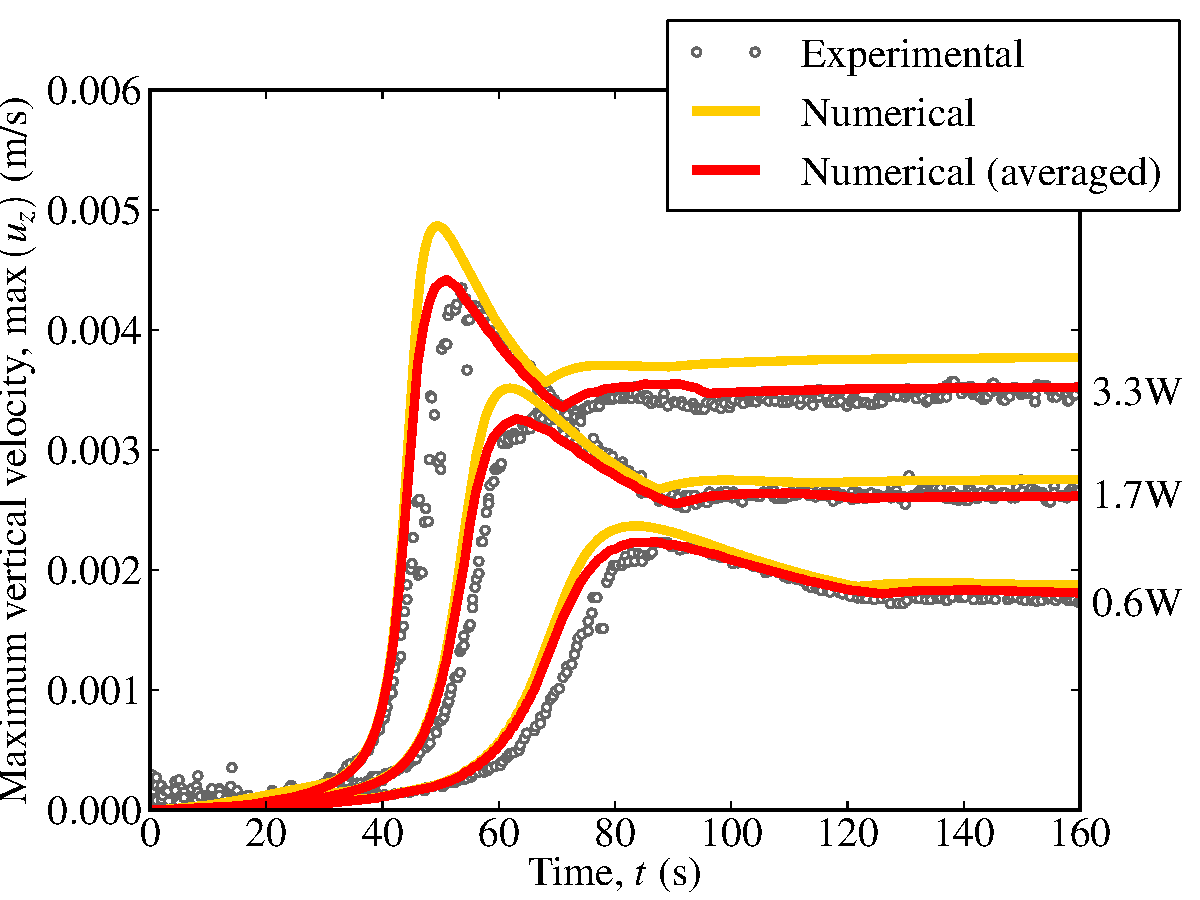
\includegraphics[width=0.47\textwidth]{data/vatteville/max_velocity} & 
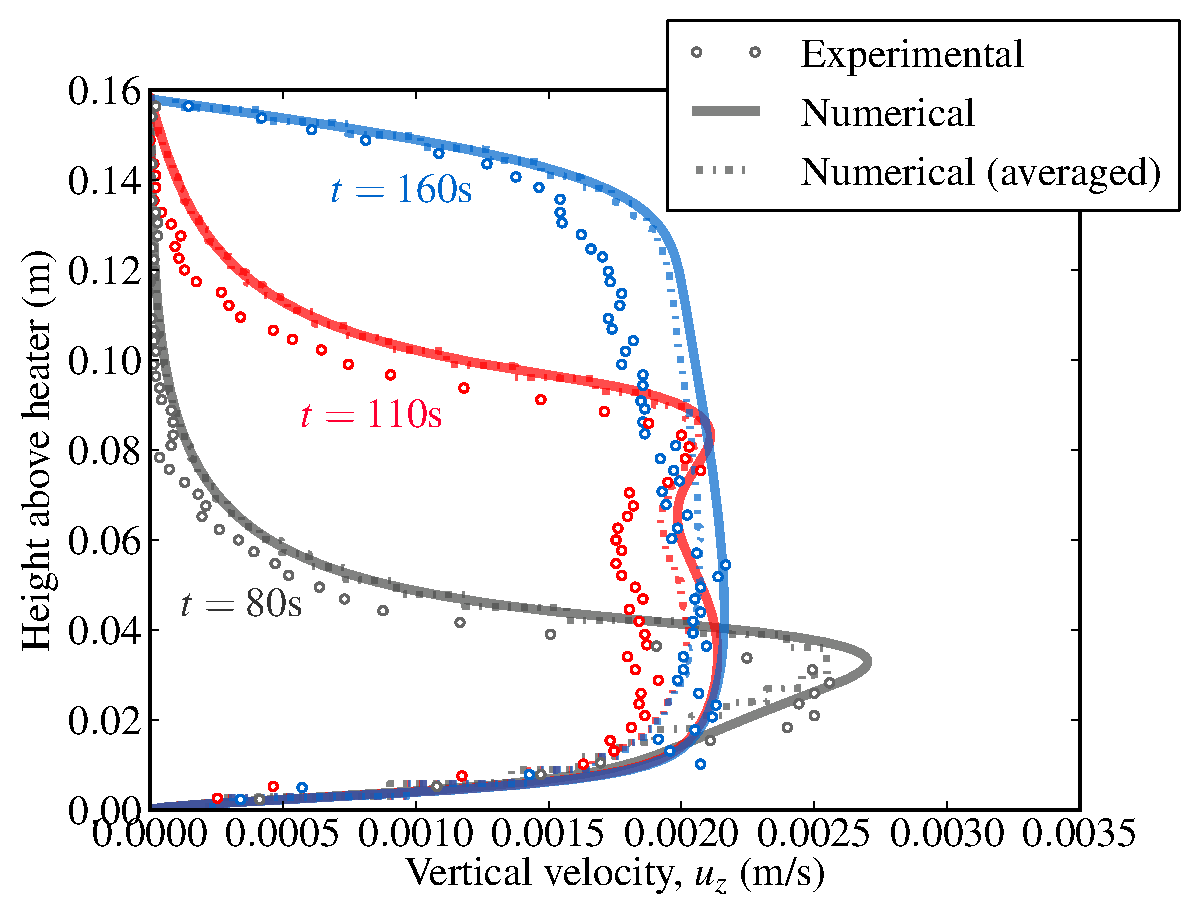
\includegraphics[width=0.47\textwidth]{data/vatteville/velocity_profile} \vspace{0.2cm} \\
\end{tabular}
\caption{(a) Benchmark results for \cite{VattevilleG32009} showing maximum velocities versus time in the laboratory experiments  and
the numerical simulations for a cylindrical plume.  Following \citet{VattevilleG32009}, the numerical data is averaged in \mm[3] squares to mimic the effect of laboratory data collection.  The effect of this averaging can also be seen in velocity profiles of the numerical 
and laboratory data above the heater (b, heater power of \W[1.0]).} 
\label{fig:vatteville}
\end{figure}




% Copyright (C) 2013 Columbia University in the City of New York and others.
%
% Please see the AUTHORS file in the main source directory for a full list
% of contributors.
%
% This file is part of TerraFERMA.
%
% TerraFERMA is free software: you can redistribute it and/or modify
% it under the terms of the GNU Lesser General Public License as published by
% the Free Software Foundation, either version 3 of the License, or
% (at your option) any later version.
%
% TerraFERMA is distributed in the hope that it will be useful,
% but WITHOUT ANY WARRANTY; without even the implied warranty of
% MERCHANTABILITY or FITNESS FOR A PARTICULAR PURPOSE. See the
% GNU Lesser General Public License for more details.
%
% You should have received a copy of the GNU Lesser General Public License
% along with TerraFERMA. If not, see <http://www.gnu.org/licenses/>.

\chapter{Compressible Two-Dimensional Convection: \citeauthor{KingGJI2010}} \label{sec:king}

\citet{KingGJI2010} defined a series of convection benchmarks similar to
those of 
\citet{BlankenbachGJI1989} 
but with a linearized
compressible equation of state.  Solutions are sought for velocity,
%PvK: you're using bold v in the main text for velocity.
$\vec{v}$, and perturbations in the temperature, $T$, and pressure $p$,
from prescribed reference states, $\bar{T}$ and $\bar{p}$
respectively, corresponding to a reference density $\bar{\rho}$.
% PvK: above is not strictly true - some of the participating codes used full T
% not just perturbation.
The importance of compressibility is indicated by the non-dimensional dissipation number 
$Di$.
%Several other parameters are also introduced leading to an enlarged
%parameter space involving both the Rayleigh, $\Ra$, and dissipation,
%$\Di$, numbers.  
Full details of the derivation can be found in
\citet{KingGJI2010} and \citet{SchubertCUP2001}.  A reduced subset of these
parameters is considered here for benchmarking purposes.  In all cases
the domain is a two-dimensional square of unit dimensions with
free-slip boundary conditions % and no normal flow boundary conditions specified on the
for the Stokes equations at all boundaries.  The side walls are insulating
(homogeneous Neumann, $\partial_x T = 0$) for temperature while $T=0$
is specified at the top surface.

\paragraph{Extended Boussinesq Approximation (EBA)}
In the extended Boussinesq approximation the velocity field remains
divergence free and  only the temperature equation sees the addition of terms that scale with the dissipation number.
% $r_T$, of the residual, $r$, is significantly modified:
% \begin{equation}
% r = r_{\dvv} + r_{p} + r_{T}
% \end{equation}
% where:
% \begin{align}
%   r_{\dvv} =& \int_\Omega \left(\frac{\nabla\dvv_t + \nabla\dvv_t^T}{2}\right) : 2
% \left(\frac{\nabla\dvv_i+\nabla\dvv_i^T}{2}\right) \nonumber \\
% &- \int_\Omega \nabla\cdot\dvv_t p_i - \int_{\Omega}(\dvv_t)_z T_i, \\
%   r_{p} =& \int_\Omega p_t\nabla\cdot \dvv_i, \\
%   r_{T} =& \int_\Omega T_t\left((T_i - T_n) + \Delta t\theta\dvv_\theta\cdot\nabla T_i + \Delta t(1-\theta)\dvv_\theta\cdot\nabla T_n\right)
% \nonumber \\
% &+\int_\Omega T_t\left(\Delta t\theta\Di(\dvv_\theta)_z T_i + \Delta t(1-\theta)\Di(\dvv_\theta)_z T_n \right)  \nonumber \\
% &+\int_\Omega T_t\left(\Delta t\Di(\dvv_\theta)_z T_0  - 2\Delta t\Di \left(\frac{\nabla\dvv_\theta + \nabla\dvv_\theta^T}{2}\right) : \nabla\dvv_\theta \right)  \nonumber \\
%  &+\int_\Omega \left(\frac{\Delta t\theta}{\Ra}\nabla T_t \nabla T_i + \frac{\Delta t(1-\theta)}{\Ra}\nabla T_t \nabla T_n\right),
% \end{align}
% and:
% \begin{equation}
% \dvv_\theta = \theta_{\dvv}\dvv_i + (1-\theta_{\dvv})\dvv_n
% \end{equation}
% and $T_0$ is the non-dimensionalized surface temperature.  
% The corresponding ufl code is given by:
% \begin{lstlisting}[language=Python]
% v_theta = theta_v*v_i + (1.-theta_v)*v_n
% recRa   = 1./Ra
%
% rv = (inner(sym(grad(v_t)), 2*sym(grad(v_i))) \
%       - div(v_t)*p_i - T_i*v_t[1] \
%      )*dx
% rp = p_t*div(v_i)*dx
% rT = (T_t*((T_i - T_n) \
%            + dt*theta*inner(v_theta, grad(T_i)) \
%            + dt*(1.-theta)*inner(v_theta, grad(T_n)) \
%            + dt*theta*Di*v_theta[1]*T_i \
%            + dt*(1.-theta)*Di*v_theta[1]*T_n \
%            + dt*Di*v_theta[1]*T0 \
%            - dt*Di*inner(2*sym(grad(v_theta)), grad(v_theta))) \
%       + dt*recRa*theta*inner(grad(T_t), grad(T_i)) \
%       + dt*recRa*(1.-theta)*inner(grad(T_t), grad(T_n)) \
%      )*dx
%
% r = rv + rp + rT
% \end{lstlisting}
An additional boundary condition for temperature, $T=1$ is applied at
the base of the domain.  Simulations are run at a variety of
resolutions, all structured but with refinement at the boundaries.
Convergence results for EBA and a range of $\Ra$ and $\Di$
can be found in Tables \ref{tab:KingEBARa1.e4}--\ref{tab:KingEBARa1.e5}.



\paragraph{Truncated Anelastic Liquid Approximation (TALA)}
A first approximation that includes the effects of compressibility in the 
Stokes equations, but ignoring the pressure effect on buoyancy is the
%Introducing a pressure dependence on density but ignoring the
%contribution this makes to buoyancy leads to the 
truncated anelastic liquid approximation (TALA).  
The velocity field now has a non-zero
divergence. % leading to a more substantial modification of the residual.
% $r$:
% \begin{equation}
% r = r_{\dvv} + r_{p} + r_{T}
% \end{equation}
% where:
% \begin{align}
%   r_{\dvv} =& \int_\Omega \left(\frac{\nabla\dvv_t + \nabla\dvv_t^T}{2}\right) : \left(2
% \left(\frac{\nabla\dvv_i+\nabla\dvv_i^T}{2}\right) - \frac{2}{3}\nabla\cdot\dvv_i\right) \nonumber \\
% &- \int_\Omega \nabla\cdot\dvv_t p_i + \int_{\Omega}\dvv_t\cdot\hat{\dvg}\bar{\rho}\bar{\alpha} T_i, \\
%   r_{p} =& \int_\Omega p_t\nabla\cdot\left(\bar{\rho}\dvv_i\right), \\
%   r_{T} =& \int_\Omega T_t\bar{\rho}\bar{c_p}\left((T_i - T_n) + \Delta t\theta\dvv_\theta\cdot\nabla T_i + \Delta t(1-\theta)\dvv_\theta\cdot\nabla T_n\right)
% \nonumber \\
% &-\int_\Omega T_t\left(\Delta t\theta\Di\dvv_\theta\cdot\hat{\dvg} T_i + \Delta t(1-\theta)\Di\dvv_\theta\cdot\hat{\dvg} T_n \right)  \nonumber \\
% &-\int_\Omega T_t\Delta t\Di \left(2\frac{\nabla\dvv_\theta + \nabla\dvv_\theta^T}{2} - \frac{2}{3}\nabla\cdot\dvv_\theta\right) : \nabla\dvv_\theta  \nonumber \\
%  &+\int_\Omega \left(\frac{\Delta t\theta}{\Ra}\nabla T_t \nabla T_i + \frac{\Delta t(1-\theta)}{\Ra}\nabla T_t \nabla T_n + \frac{\Delta
% t}{\Ra}\nabla T_t \nabla \bar{T}\right),
% \end{align}
% and:
% \begin{align}
% \bar{\rho} =& \exp\left(\frac{(1-z)\Di}{\gamma_r}\right) \\
% \bar{T} =& T_\text{surf}\exp\left((1-z)\Di\right) - T_\text{surf} \\
% \bar{\alpha} =& 1 \\
% \bar{c_p} =& 1 \\
% \bar{\chi} =& 1 \\
% \dvv_\theta =& \theta_{\dvv}\dvv_i + (1-\theta_{\dvv})\dvv_n.
% \end{align}
% The corresponding ufl code is given by:
% \begin{lstlisting}[language=Python]
% rhobar   = exp(depth*Di/gammar) 
% Tbar     = Tsurf*exp(Di*depth) - Tsurf 
% alphabar = 1.0
% cpbar    = 1.0
% Chibar   = 1.0
%
% v_theta  = theta_v*v_i + (1.-theta_v)*v_n
% recRa    = 1./Ra
%
% I = Identity(dim)
% def stress(v):
%   return 2*sym(grad(v))-0.666666666666666*I*div(v)
%
% rv = (inner(sym(grad(v_t)), stress(v_i)) - div(v_t)*p_i \
%       + inner(v_t, gravity)*rhobar*alphabar*T_i \
%      )*dx
% rp = p_t*div(rhobar*v_i)*dx
% rT = (T_t*(rhobar*cpbar*((T_i - T_n) \
%                          + dt*theta*inner(v_theta, grad(T_i)) \
%                          + dt*(1.-theta)*inner(v_theta, grad(T_n))) \
%            - dt*theta*Di*inner(v_theta, gravity)*alphabar*rhobar*T_i \
%            - dt*(1.-theta)*Di*inner(v_theta, gravity)*alphabar*rhobar*T_n \
%            - dt*Di*inner(stress(v_theta), grad(v_theta))) \
%       + dt*recRa*theta*inner(grad(T_t), grad(T_i)) \
%       + dt*recRa*(1.-theta)*inner(grad(T_t), grad(T_n)) \
%       + dt*recRa*inner(grad(T_t), grad(Tbar))\
%      )*dx
%
% r = rv + rp + rT
% \end{lstlisting}
Since we solve our equations in potential temperature we use a modified 
temperature condition at the lower boundary, which is now given 
%At the base of the domain the temperature boundary condition is given
by $T = 1 + T_0\left(1 - \exp(\Di)\right)$.  Simulations are run at a
variety of resolutions, all structured but with refinement at the
boundaries.  Convergence results for TALA for a range of
$\Ra$, and $\Di$  can be found in Tables \ref{tab:KingTALARa1.e4}--\ref{tab:KingTALARa1.e5}.


\paragraph{Anelastic Liquid Approximation (ALA)}
In the anelastic liquid approximation (ALA) the effects of the
pressure on buoyancy are now included. % in the velocity residual.
% , $r_{\dvv}$:
% \begin{align}
%   r_{\dvv} =& \int_\Omega \left(\frac{\nabla\dvv_t + \nabla\dvv_t^T}{2}\right) : \left(2
% \left(\frac{\nabla\dvv_i+\nabla\dvv_i^T}{2}\right) - \frac{2}{3}\nabla\cdot\dvv_i\right) \nonumber \\
% &- \int_\Omega \nabla\cdot\dvv_t p_i + \int_{\Omega}\dvv_t\cdot\hat{\dvg}\left(\bar{\rho}\bar{\alpha} T_i -
% \frac{\Di}{\gamma_r}\frac{c_{p_r}}{c_{v_r}}\bar{\rho}\bar{\chi}p_i\right) 
% \end{align}
% leading only to a small modification of the ufl code:
% \begin{lstlisting}[language=Python]
% rv = (inner(sym(grad(v_t)), stress(v_i)) - div(v_t)*p_i \
%       + inner(v_t, gravity)*(rhobar*alphabar*T_i  \
%                              - (Di/gammar)*(cpr/cvr)*rhobar*Chibar*p_i)\
%      )*dx
% \end{lstlisting}
As in TALA the temperature at the base of the domain is given by $T =
1 + T_0\left(1 - \exp(\Di)\right)$.  Simulations are run at a variety
of resolutions, all structured but with refinement at the boundaries.
Convergence results for ALA for a range of
$\Ra$, and $\Di$  can be found in Tables \ref{tab:KingALARa1.e4}--\ref{tab:kingalaRa5.e5Di0.25}.



\paragraph{Temperature Dependent Viscosity ALA}
One set of benchmarks uses the same temperature-dependence of
viscosity as in the \citet{BlankenbachGJI1989} case 2a.
%Introducing a temperature dependent viscosity also only modifies the velocity residual, $r_v$, such that:
%\begin{align}
%  r_{\dvv} =& \int_\Omega \left(\frac{\nabla\dvv_t + \nabla\dvv_t^T}{2}\right) : \left(2\mu
%\left(\frac{\nabla\dvv_i+\nabla\dvv_i^T}{2}\right) - \frac{2}{3}\nabla\cdot\dvv_i\right) \nonumber \\
%&- \int_\Omega \nabla\cdot\dvv_t p_i + \int_{\Omega}\dvv_t\cdot\hat{\dvg}\left(\bar{\rho}\bar{\alpha} T_i -
%\frac{\Di}{\gamma_r}\frac{c_{p_r}}{c_{v_r}}\bar{\rho}\bar{\chi}p_i\right)
%\end{align}
%where:
%\begin{equation}
% \mu = \exp\left(-bT_i\right).
%\end{equation}
% Leading to a small modification of the underlying ufl code:
% \begin{lstlisting}[language=Python]
% b = 6.9077552789821368
% mu = exp(-b*T_i)
%
% def stress(v):
%   return 2*mu*sym(grad(v))-0.666666666666666*I*mu*div(v)
% \end{lstlisting}
Simulations are run at a variety of resolutions, all structured but
with refinement at the boundaries.  Convergence results for  a range
of $\Ra$, and $\Di$  can be found in Table \ref{tab:KingTdepALARa1.e4}.

\begin{table*}[h]
\caption{Results from 2D, isoviscous square convection benchmark
  cases using the extended Bousinesq approximation (EBA) at
  $\Ra = 10^{4}$ \citep{KingGJI2010}}  
\begin{center}
  \begin{tabular}{ll}
\fbox{\begin{minipage}[c]{0.025\textwidth}\begin{sideways}$\Di = 0.25$\end{sideways}\end{minipage}} 
&
\fbox{\begin{minipage}[c]{0.915\textwidth}\begin{tabular}{cccc}
     $N$ & $c\Delta t/\delta$  & $||\epsilon_{\phi}||$ & $\epsilon_{c}$  \\
32$\times$32 & 2.00 & 1.427786e-02 & 1.182138e-02  \\
32$\times$32 & 1.00 & 3.819159e-03 & 3.255477e-03  \\
32$\times$32 & 0.50 & 1.634865e-03 & 8.485232e-04  \\
32$\times$32 & 0.25 & 2.202831e-03 & 3.357135e-04  \\
64$\times$64 & 2.00 & 1.424202e-02 & 1.188175e-02  \\
64$\times$64 & 1.00 & 3.690917e-03 & 3.187174e-03  \\
64$\times$64 & 0.50 & 9.481209e-04 & 8.235713e-04  \\
64$\times$64 & 0.25 & 4.243532e-04 & 1.921914e-04  \\
128$\times$128 & 2.00 & 1.424087e-02 & 1.188190e-02  \\
128$\times$128 & 1.00 & 3.686779e-03 & 3.194658e-03  \\
128$\times$128 & 0.50 & 9.306871e-04 & 8.119311e-04  \\
128$\times$128 & 0.25 & 2.365556e-04 & 2.073026e-04  \\
\end{tabular}
\end{minipage}} \\
\\
\fbox{\begin{minipage}[c]{0.025\textwidth}\begin{sideways}$\Di = 0.5$\end{sideways}\end{minipage}} 
&
\fbox{\begin{minipage}[c]{0.915\textwidth}\begin{tabular}{cccc}
     $N$ & $c\Delta t/\delta$  & $||\epsilon_{\phi}||$ & $\epsilon_{c}$  \\
32$\times$32 & 2.00 & 1.427786e-02 & 1.182138e-02  \\
32$\times$32 & 1.00 & 3.819159e-03 & 3.255477e-03  \\
32$\times$32 & 0.50 & 1.634865e-03 & 8.485232e-04  \\
32$\times$32 & 0.25 & 2.202831e-03 & 3.357135e-04  \\
64$\times$64 & 2.00 & 1.424202e-02 & 1.188175e-02  \\
64$\times$64 & 1.00 & 3.690917e-03 & 3.187174e-03  \\
64$\times$64 & 0.50 & 9.481209e-04 & 8.235713e-04  \\
64$\times$64 & 0.25 & 4.243532e-04 & 1.921914e-04  \\
128$\times$128 & 2.00 & 1.424087e-02 & 1.188190e-02  \\
128$\times$128 & 1.00 & 3.686779e-03 & 3.194658e-03  \\
128$\times$128 & 0.50 & 9.306871e-04 & 8.119311e-04  \\
128$\times$128 & 0.25 & 2.365556e-04 & 2.073026e-04  \\
\end{tabular}
\end{minipage}} \\
\\
\fbox{\begin{minipage}[c]{0.025\textwidth}\begin{sideways}$\Di = 1.0$\end{sideways}\end{minipage}} 
&
\fbox{\begin{minipage}[c]{0.915\textwidth}\begin{tabular}{cccc}
     $N$ & $c\Delta t/\delta$  & $||\epsilon_{\phi}||$ & $\epsilon_{c}$  \\
32$\times$32 & 2.00 & 1.427786e-02 & 1.182138e-02  \\
32$\times$32 & 1.00 & 3.819159e-03 & 3.255477e-03  \\
32$\times$32 & 0.50 & 1.634865e-03 & 8.485232e-04  \\
32$\times$32 & 0.25 & 2.202831e-03 & 3.357135e-04  \\
64$\times$64 & 2.00 & 1.424202e-02 & 1.188175e-02  \\
64$\times$64 & 1.00 & 3.690917e-03 & 3.187174e-03  \\
64$\times$64 & 0.50 & 9.481209e-04 & 8.235713e-04  \\
64$\times$64 & 0.25 & 4.243532e-04 & 1.921914e-04  \\
128$\times$128 & 2.00 & 1.424087e-02 & 1.188190e-02  \\
128$\times$128 & 1.00 & 3.686779e-03 & 3.194658e-03  \\
128$\times$128 & 0.50 & 9.306871e-04 & 8.119311e-04  \\
128$\times$128 & 0.25 & 2.365556e-04 & 2.073026e-04  \\
\end{tabular}
\end{minipage}}
  \end{tabular}
\end{center}
  \label{tab:KingEBARa1.e4}
\end{table*}

\begin{table*}[h]
\caption{Results from 2D, isoviscous square convection benchmark
  cases using the extended Bousinesq approximation (EBA) at
  $\Ra = 10^{5}$ \citep{KingGJI2010}}  
\begin{center}
  \begin{tabular}{ll}
\fbox{\begin{minipage}[c]{0.025\textwidth}\begin{sideways}$\Di = 0.25$\end{sideways}\end{minipage}} 
&
\fbox{\begin{minipage}[c]{0.915\textwidth}\begin{tabular}{cccc}
     $N$ & $c\Delta t/\delta$  & $||\epsilon_{\phi}||$ & $\epsilon_{c}$  \\
32$\times$32 & 2.00 & 1.427786e-02 & 1.182138e-02  \\
32$\times$32 & 1.00 & 3.819159e-03 & 3.255477e-03  \\
32$\times$32 & 0.50 & 1.634865e-03 & 8.485232e-04  \\
32$\times$32 & 0.25 & 2.202831e-03 & 3.357135e-04  \\
64$\times$64 & 2.00 & 1.424202e-02 & 1.188175e-02  \\
64$\times$64 & 1.00 & 3.690917e-03 & 3.187174e-03  \\
64$\times$64 & 0.50 & 9.481209e-04 & 8.235713e-04  \\
64$\times$64 & 0.25 & 4.243532e-04 & 1.921914e-04  \\
128$\times$128 & 2.00 & 1.424087e-02 & 1.188190e-02  \\
128$\times$128 & 1.00 & 3.686779e-03 & 3.194658e-03  \\
128$\times$128 & 0.50 & 9.306871e-04 & 8.119311e-04  \\
128$\times$128 & 0.25 & 2.365556e-04 & 2.073026e-04  \\
\end{tabular}
\end{minipage}} \\
\\
\fbox{\begin{minipage}[c]{0.025\textwidth}\begin{sideways}$\Di = 0.5$\end{sideways}\end{minipage}} 
&
\fbox{\begin{minipage}[c]{0.915\textwidth}\begin{tabular}{cccc}
     $N$ & $c\Delta t/\delta$  & $||\epsilon_{\phi}||$ & $\epsilon_{c}$  \\
32$\times$32 & 2.00 & 1.427786e-02 & 1.182138e-02  \\
32$\times$32 & 1.00 & 3.819159e-03 & 3.255477e-03  \\
32$\times$32 & 0.50 & 1.634865e-03 & 8.485232e-04  \\
32$\times$32 & 0.25 & 2.202831e-03 & 3.357135e-04  \\
64$\times$64 & 2.00 & 1.424202e-02 & 1.188175e-02  \\
64$\times$64 & 1.00 & 3.690917e-03 & 3.187174e-03  \\
64$\times$64 & 0.50 & 9.481209e-04 & 8.235713e-04  \\
64$\times$64 & 0.25 & 4.243532e-04 & 1.921914e-04  \\
128$\times$128 & 2.00 & 1.424087e-02 & 1.188190e-02  \\
128$\times$128 & 1.00 & 3.686779e-03 & 3.194658e-03  \\
128$\times$128 & 0.50 & 9.306871e-04 & 8.119311e-04  \\
128$\times$128 & 0.25 & 2.365556e-04 & 2.073026e-04  \\
\end{tabular}
\end{minipage}} \\
\\
\fbox{\begin{minipage}[c]{0.025\textwidth}\begin{sideways}$\Di = 1.0$\end{sideways}\end{minipage}} 
&
\fbox{\begin{minipage}[c]{0.915\textwidth}\begin{tabular}{cccc}
     $N$ & $c\Delta t/\delta$  & $||\epsilon_{\phi}||$ & $\epsilon_{c}$  \\
32$\times$32 & 2.00 & 1.427786e-02 & 1.182138e-02  \\
32$\times$32 & 1.00 & 3.819159e-03 & 3.255477e-03  \\
32$\times$32 & 0.50 & 1.634865e-03 & 8.485232e-04  \\
32$\times$32 & 0.25 & 2.202831e-03 & 3.357135e-04  \\
64$\times$64 & 2.00 & 1.424202e-02 & 1.188175e-02  \\
64$\times$64 & 1.00 & 3.690917e-03 & 3.187174e-03  \\
64$\times$64 & 0.50 & 9.481209e-04 & 8.235713e-04  \\
64$\times$64 & 0.25 & 4.243532e-04 & 1.921914e-04  \\
128$\times$128 & 2.00 & 1.424087e-02 & 1.188190e-02  \\
128$\times$128 & 1.00 & 3.686779e-03 & 3.194658e-03  \\
128$\times$128 & 0.50 & 9.306871e-04 & 8.119311e-04  \\
128$\times$128 & 0.25 & 2.365556e-04 & 2.073026e-04  \\
\end{tabular}
\end{minipage}}
  \end{tabular}
\end{center}
  \label{tab:KingEBARa1.e5}
\end{table*}



\begin{table*}[h]
\caption{Results from 2D, isoviscous square convection benchmark
  cases using the truncated anelastic approximation (TALA) at $\Ra = 10^{4}$  \citep{KingGJI2010}}  
\begin{center}
  \begin{tabular}{ll}
\fbox{\begin{minipage}[c]{0.025\textwidth}\begin{sideways}$\Di = 0.25$\end{sideways}\end{minipage}} 
&
\fbox{\begin{minipage}[c]{0.915\textwidth}\begin{tabular}{cccc}
     $N$ & $c\Delta t/\delta$  & $||\epsilon_{\phi}||$ & $\epsilon_{c}$  \\
32$\times$32 & 2.00 & 1.427786e-02 & 1.182138e-02  \\
32$\times$32 & 1.00 & 3.819159e-03 & 3.255477e-03  \\
32$\times$32 & 0.50 & 1.634865e-03 & 8.485232e-04  \\
32$\times$32 & 0.25 & 2.202831e-03 & 3.357135e-04  \\
64$\times$64 & 2.00 & 1.424202e-02 & 1.188175e-02  \\
64$\times$64 & 1.00 & 3.690917e-03 & 3.187174e-03  \\
64$\times$64 & 0.50 & 9.481209e-04 & 8.235713e-04  \\
64$\times$64 & 0.25 & 4.243532e-04 & 1.921914e-04  \\
128$\times$128 & 2.00 & 1.424087e-02 & 1.188190e-02  \\
128$\times$128 & 1.00 & 3.686779e-03 & 3.194658e-03  \\
128$\times$128 & 0.50 & 9.306871e-04 & 8.119311e-04  \\
128$\times$128 & 0.25 & 2.365556e-04 & 2.073026e-04  \\
\end{tabular}
\end{minipage}} \\
\\
\fbox{\begin{minipage}[c]{0.025\textwidth}\begin{sideways}$\Di = 1.0$\end{sideways}\end{minipage}} 
&
\fbox{\begin{minipage}[c]{0.915\textwidth}\begin{tabular}{cccc}
     $N$ & $c\Delta t/\delta$  & $||\epsilon_{\phi}||$ & $\epsilon_{c}$  \\
32$\times$32 & 2.00 & 1.427786e-02 & 1.182138e-02  \\
32$\times$32 & 1.00 & 3.819159e-03 & 3.255477e-03  \\
32$\times$32 & 0.50 & 1.634865e-03 & 8.485232e-04  \\
32$\times$32 & 0.25 & 2.202831e-03 & 3.357135e-04  \\
64$\times$64 & 2.00 & 1.424202e-02 & 1.188175e-02  \\
64$\times$64 & 1.00 & 3.690917e-03 & 3.187174e-03  \\
64$\times$64 & 0.50 & 9.481209e-04 & 8.235713e-04  \\
64$\times$64 & 0.25 & 4.243532e-04 & 1.921914e-04  \\
128$\times$128 & 2.00 & 1.424087e-02 & 1.188190e-02  \\
128$\times$128 & 1.00 & 3.686779e-03 & 3.194658e-03  \\
128$\times$128 & 0.50 & 9.306871e-04 & 8.119311e-04  \\
128$\times$128 & 0.25 & 2.365556e-04 & 2.073026e-04  \\
\end{tabular}
\end{minipage}} \\
\\
\fbox{\begin{minipage}[c]{0.025\textwidth}\begin{sideways}$\Di = 1.5$\end{sideways}\end{minipage}} 
&
\fbox{\begin{minipage}[c]{0.915\textwidth}\begin{tabular}{cccc}
     $N$ & $c\Delta t/\delta$  & $||\epsilon_{\phi}||$ & $\epsilon_{c}$  \\
32$\times$32 & 2.00 & 1.427786e-02 & 1.182138e-02  \\
32$\times$32 & 1.00 & 3.819159e-03 & 3.255477e-03  \\
32$\times$32 & 0.50 & 1.634865e-03 & 8.485232e-04  \\
32$\times$32 & 0.25 & 2.202831e-03 & 3.357135e-04  \\
64$\times$64 & 2.00 & 1.424202e-02 & 1.188175e-02  \\
64$\times$64 & 1.00 & 3.690917e-03 & 3.187174e-03  \\
64$\times$64 & 0.50 & 9.481209e-04 & 8.235713e-04  \\
64$\times$64 & 0.25 & 4.243532e-04 & 1.921914e-04  \\
128$\times$128 & 2.00 & 1.424087e-02 & 1.188190e-02  \\
128$\times$128 & 1.00 & 3.686779e-03 & 3.194658e-03  \\
128$\times$128 & 0.50 & 9.306871e-04 & 8.119311e-04  \\
128$\times$128 & 0.25 & 2.365556e-04 & 2.073026e-04  \\
\end{tabular}
\end{minipage}}
  \end{tabular}
\end{center}
  \label{tab:KingTALARa1.e4}
\end{table*}

\begin{table*}[h]
\caption{Results from 2D, isoviscous square convection benchmark
  cases using the truncated anelastic approximation (TALA) at $\Ra = 10^{5}$ \citep{KingGJI2010}}  
\begin{center}
  \begin{tabular}{ll}
\fbox{\begin{minipage}[c]{0.025\textwidth}\begin{sideways}$\Di = 0.25$\end{sideways}\end{minipage}} 
&
\fbox{\begin{minipage}[c]{0.915\textwidth}\begin{tabular}{cccc}
     $N$ & $c\Delta t/\delta$  & $||\epsilon_{\phi}||$ & $\epsilon_{c}$  \\
32$\times$32 & 2.00 & 1.427786e-02 & 1.182138e-02  \\
32$\times$32 & 1.00 & 3.819159e-03 & 3.255477e-03  \\
32$\times$32 & 0.50 & 1.634865e-03 & 8.485232e-04  \\
32$\times$32 & 0.25 & 2.202831e-03 & 3.357135e-04  \\
64$\times$64 & 2.00 & 1.424202e-02 & 1.188175e-02  \\
64$\times$64 & 1.00 & 3.690917e-03 & 3.187174e-03  \\
64$\times$64 & 0.50 & 9.481209e-04 & 8.235713e-04  \\
64$\times$64 & 0.25 & 4.243532e-04 & 1.921914e-04  \\
128$\times$128 & 2.00 & 1.424087e-02 & 1.188190e-02  \\
128$\times$128 & 1.00 & 3.686779e-03 & 3.194658e-03  \\
128$\times$128 & 0.50 & 9.306871e-04 & 8.119311e-04  \\
128$\times$128 & 0.25 & 2.365556e-04 & 2.073026e-04  \\
\end{tabular}
\end{minipage}} \\
\\
\fbox{\begin{minipage}[c]{0.025\textwidth}\begin{sideways}$\Di = 1.0$\end{sideways}\end{minipage}} 
&
\fbox{\begin{minipage}[c]{0.915\textwidth}\begin{tabular}{cccc}
     $N$ & $c\Delta t/\delta$  & $||\epsilon_{\phi}||$ & $\epsilon_{c}$  \\
32$\times$32 & 2.00 & 1.427786e-02 & 1.182138e-02  \\
32$\times$32 & 1.00 & 3.819159e-03 & 3.255477e-03  \\
32$\times$32 & 0.50 & 1.634865e-03 & 8.485232e-04  \\
32$\times$32 & 0.25 & 2.202831e-03 & 3.357135e-04  \\
64$\times$64 & 2.00 & 1.424202e-02 & 1.188175e-02  \\
64$\times$64 & 1.00 & 3.690917e-03 & 3.187174e-03  \\
64$\times$64 & 0.50 & 9.481209e-04 & 8.235713e-04  \\
64$\times$64 & 0.25 & 4.243532e-04 & 1.921914e-04  \\
128$\times$128 & 2.00 & 1.424087e-02 & 1.188190e-02  \\
128$\times$128 & 1.00 & 3.686779e-03 & 3.194658e-03  \\
128$\times$128 & 0.50 & 9.306871e-04 & 8.119311e-04  \\
128$\times$128 & 0.25 & 2.365556e-04 & 2.073026e-04  \\
\end{tabular}
\end{minipage}} \\
\\
\fbox{\begin{minipage}[c]{0.025\textwidth}\begin{sideways}$\Di = 1.5$\end{sideways}\end{minipage}} 
&
\fbox{\begin{minipage}[c]{0.915\textwidth}\begin{tabular}{cccc}
     $N$ & $c\Delta t/\delta$  & $||\epsilon_{\phi}||$ & $\epsilon_{c}$  \\
32$\times$32 & 2.00 & 1.427786e-02 & 1.182138e-02  \\
32$\times$32 & 1.00 & 3.819159e-03 & 3.255477e-03  \\
32$\times$32 & 0.50 & 1.634865e-03 & 8.485232e-04  \\
32$\times$32 & 0.25 & 2.202831e-03 & 3.357135e-04  \\
64$\times$64 & 2.00 & 1.424202e-02 & 1.188175e-02  \\
64$\times$64 & 1.00 & 3.690917e-03 & 3.187174e-03  \\
64$\times$64 & 0.50 & 9.481209e-04 & 8.235713e-04  \\
64$\times$64 & 0.25 & 4.243532e-04 & 1.921914e-04  \\
128$\times$128 & 2.00 & 1.424087e-02 & 1.188190e-02  \\
128$\times$128 & 1.00 & 3.686779e-03 & 3.194658e-03  \\
128$\times$128 & 0.50 & 9.306871e-04 & 8.119311e-04  \\
128$\times$128 & 0.25 & 2.365556e-04 & 2.073026e-04  \\
\end{tabular}
\end{minipage}}
  \end{tabular}
\end{center}
  \label{tab:KingTALARa1.e5}
\end{table*}

\begin{table*}[h]
\caption{Results from 2D, isoviscous square convection benchmark
  cases using the anelastic liquid approximation (ALA) at $\Ra = 10^{4}$  \citep{KingGJI2010}}  
\begin{center}
  \begin{tabular}{ll}
\fbox{\begin{minipage}[c]{0.025\textwidth}\begin{sideways}$\Di = 0.25$\end{sideways}\end{minipage}} 
&
\fbox{\begin{minipage}[c]{0.915\textwidth}\begin{tabular}{cccc}
     $N$ & $c\Delta t/\delta$  & $||\epsilon_{\phi}||$ & $\epsilon_{c}$  \\
32$\times$32 & 2.00 & 1.427786e-02 & 1.182138e-02  \\
32$\times$32 & 1.00 & 3.819159e-03 & 3.255477e-03  \\
32$\times$32 & 0.50 & 1.634865e-03 & 8.485232e-04  \\
32$\times$32 & 0.25 & 2.202831e-03 & 3.357135e-04  \\
64$\times$64 & 2.00 & 1.424202e-02 & 1.188175e-02  \\
64$\times$64 & 1.00 & 3.690917e-03 & 3.187174e-03  \\
64$\times$64 & 0.50 & 9.481209e-04 & 8.235713e-04  \\
64$\times$64 & 0.25 & 4.243532e-04 & 1.921914e-04  \\
128$\times$128 & 2.00 & 1.424087e-02 & 1.188190e-02  \\
128$\times$128 & 1.00 & 3.686779e-03 & 3.194658e-03  \\
128$\times$128 & 0.50 & 9.306871e-04 & 8.119311e-04  \\
128$\times$128 & 0.25 & 2.365556e-04 & 2.073026e-04  \\
\end{tabular}
\end{minipage}} \\
\\
\fbox{\begin{minipage}[c]{0.025\textwidth}\begin{sideways}$\Di = 1.0$\end{sideways}\end{minipage}} 
&
\fbox{\begin{minipage}[c]{0.915\textwidth}\begin{tabular}{cccc}
     $N$ & $c\Delta t/\delta$  & $||\epsilon_{\phi}||$ & $\epsilon_{c}$  \\
32$\times$32 & 2.00 & 1.427786e-02 & 1.182138e-02  \\
32$\times$32 & 1.00 & 3.819159e-03 & 3.255477e-03  \\
32$\times$32 & 0.50 & 1.634865e-03 & 8.485232e-04  \\
32$\times$32 & 0.25 & 2.202831e-03 & 3.357135e-04  \\
64$\times$64 & 2.00 & 1.424202e-02 & 1.188175e-02  \\
64$\times$64 & 1.00 & 3.690917e-03 & 3.187174e-03  \\
64$\times$64 & 0.50 & 9.481209e-04 & 8.235713e-04  \\
64$\times$64 & 0.25 & 4.243532e-04 & 1.921914e-04  \\
128$\times$128 & 2.00 & 1.424087e-02 & 1.188190e-02  \\
128$\times$128 & 1.00 & 3.686779e-03 & 3.194658e-03  \\
128$\times$128 & 0.50 & 9.306871e-04 & 8.119311e-04  \\
128$\times$128 & 0.25 & 2.365556e-04 & 2.073026e-04  \\
\end{tabular}
\end{minipage}} \\
\\
\fbox{\begin{minipage}[c]{0.025\textwidth}\begin{sideways}$\Di = 1.5$\end{sideways}\end{minipage}} 
&
\fbox{\begin{minipage}[c]{0.915\textwidth}\begin{tabular}{cccc}
     $N$ & $c\Delta t/\delta$  & $||\epsilon_{\phi}||$ & $\epsilon_{c}$  \\
32$\times$32 & 2.00 & 1.427786e-02 & 1.182138e-02  \\
32$\times$32 & 1.00 & 3.819159e-03 & 3.255477e-03  \\
32$\times$32 & 0.50 & 1.634865e-03 & 8.485232e-04  \\
32$\times$32 & 0.25 & 2.202831e-03 & 3.357135e-04  \\
64$\times$64 & 2.00 & 1.424202e-02 & 1.188175e-02  \\
64$\times$64 & 1.00 & 3.690917e-03 & 3.187174e-03  \\
64$\times$64 & 0.50 & 9.481209e-04 & 8.235713e-04  \\
64$\times$64 & 0.25 & 4.243532e-04 & 1.921914e-04  \\
128$\times$128 & 2.00 & 1.424087e-02 & 1.188190e-02  \\
128$\times$128 & 1.00 & 3.686779e-03 & 3.194658e-03  \\
128$\times$128 & 0.50 & 9.306871e-04 & 8.119311e-04  \\
128$\times$128 & 0.25 & 2.365556e-04 & 2.073026e-04  \\
\end{tabular}
\end{minipage}}
  \end{tabular}
\end{center}
  \label{tab:KingALARa1.e4}
\end{table*}

\begin{table*}[h]
\caption{Results from 2D, isoviscous square convection benchmark
  cases using the anelastic liquid approximation (ALA) at $\Ra = 10^{5}$  \citep{KingGJI2010}}  
\begin{center}
  \begin{tabular}{ll}
\fbox{\begin{minipage}[c]{0.025\textwidth}\begin{sideways}$\Di = 0.25$\end{sideways}\end{minipage}} 
&
\fbox{\begin{minipage}[c]{0.915\textwidth}\begin{tabular}{cccc}
     $N$ & $c\Delta t/\delta$  & $||\epsilon_{\phi}||$ & $\epsilon_{c}$  \\
32$\times$32 & 2.00 & 1.427786e-02 & 1.182138e-02  \\
32$\times$32 & 1.00 & 3.819159e-03 & 3.255477e-03  \\
32$\times$32 & 0.50 & 1.634865e-03 & 8.485232e-04  \\
32$\times$32 & 0.25 & 2.202831e-03 & 3.357135e-04  \\
64$\times$64 & 2.00 & 1.424202e-02 & 1.188175e-02  \\
64$\times$64 & 1.00 & 3.690917e-03 & 3.187174e-03  \\
64$\times$64 & 0.50 & 9.481209e-04 & 8.235713e-04  \\
64$\times$64 & 0.25 & 4.243532e-04 & 1.921914e-04  \\
128$\times$128 & 2.00 & 1.424087e-02 & 1.188190e-02  \\
128$\times$128 & 1.00 & 3.686779e-03 & 3.194658e-03  \\
128$\times$128 & 0.50 & 9.306871e-04 & 8.119311e-04  \\
128$\times$128 & 0.25 & 2.365556e-04 & 2.073026e-04  \\
\end{tabular}
\end{minipage}} \\
\\
\fbox{\begin{minipage}[c]{0.025\textwidth}\begin{sideways}$\Di = 1.0$\end{sideways}\end{minipage}} 
&
\fbox{\begin{minipage}[c]{0.915\textwidth}\begin{tabular}{cccc}
     $N$ & $c\Delta t/\delta$  & $||\epsilon_{\phi}||$ & $\epsilon_{c}$  \\
32$\times$32 & 2.00 & 1.427786e-02 & 1.182138e-02  \\
32$\times$32 & 1.00 & 3.819159e-03 & 3.255477e-03  \\
32$\times$32 & 0.50 & 1.634865e-03 & 8.485232e-04  \\
32$\times$32 & 0.25 & 2.202831e-03 & 3.357135e-04  \\
64$\times$64 & 2.00 & 1.424202e-02 & 1.188175e-02  \\
64$\times$64 & 1.00 & 3.690917e-03 & 3.187174e-03  \\
64$\times$64 & 0.50 & 9.481209e-04 & 8.235713e-04  \\
64$\times$64 & 0.25 & 4.243532e-04 & 1.921914e-04  \\
128$\times$128 & 2.00 & 1.424087e-02 & 1.188190e-02  \\
128$\times$128 & 1.00 & 3.686779e-03 & 3.194658e-03  \\
128$\times$128 & 0.50 & 9.306871e-04 & 8.119311e-04  \\
128$\times$128 & 0.25 & 2.365556e-04 & 2.073026e-04  \\
\end{tabular}
\end{minipage}} \\
\\
\fbox{\begin{minipage}[c]{0.025\textwidth}\begin{sideways}$\Di = 1.5$\end{sideways}\end{minipage}} 
&
\fbox{\begin{minipage}[c]{0.915\textwidth}\begin{tabular}{cccc}
     $N$ & $c\Delta t/\delta$  & $||\epsilon_{\phi}||$ & $\epsilon_{c}$  \\
32$\times$32 & 2.00 & 1.427786e-02 & 1.182138e-02  \\
32$\times$32 & 1.00 & 3.819159e-03 & 3.255477e-03  \\
32$\times$32 & 0.50 & 1.634865e-03 & 8.485232e-04  \\
32$\times$32 & 0.25 & 2.202831e-03 & 3.357135e-04  \\
64$\times$64 & 2.00 & 1.424202e-02 & 1.188175e-02  \\
64$\times$64 & 1.00 & 3.690917e-03 & 3.187174e-03  \\
64$\times$64 & 0.50 & 9.481209e-04 & 8.235713e-04  \\
64$\times$64 & 0.25 & 4.243532e-04 & 1.921914e-04  \\
128$\times$128 & 2.00 & 1.424087e-02 & 1.188190e-02  \\
128$\times$128 & 1.00 & 3.686779e-03 & 3.194658e-03  \\
128$\times$128 & 0.50 & 9.306871e-04 & 8.119311e-04  \\
128$\times$128 & 0.25 & 2.365556e-04 & 2.073026e-04  \\
\end{tabular}
\end{minipage}}
  \end{tabular}
\end{center}
  \label{tab:KingALARa1.e5}
\end{table*}

\begin{table*}[h]
\caption{Results from 2D, isoviscous square convection benchmark
  cases using the anelastic approximation (ALA) at $\Ra = 5
\times 10^{5}$ \citep{KingGJI2010}.} 
\begin{center}
  \begin{tabular}{ll}
\fbox{\begin{minipage}[c]{0.025\textwidth}\begin{sideways}$\Di = 0.25$\end{sideways}\end{minipage}} 
&
\fbox{\begin{minipage}[c]{0.925\textwidth}\begin{tabular}{cccc}
     $N$ & $c\Delta t/\delta$  & $||\epsilon_{\phi}||$ & $\epsilon_{c}$  \\
32$\times$32 & 2.00 & 1.427786e-02 & 1.182138e-02  \\
32$\times$32 & 1.00 & 3.819159e-03 & 3.255477e-03  \\
32$\times$32 & 0.50 & 1.634865e-03 & 8.485232e-04  \\
32$\times$32 & 0.25 & 2.202831e-03 & 3.357135e-04  \\
64$\times$64 & 2.00 & 1.424202e-02 & 1.188175e-02  \\
64$\times$64 & 1.00 & 3.690917e-03 & 3.187174e-03  \\
64$\times$64 & 0.50 & 9.481209e-04 & 8.235713e-04  \\
64$\times$64 & 0.25 & 4.243532e-04 & 1.921914e-04  \\
128$\times$128 & 2.00 & 1.424087e-02 & 1.188190e-02  \\
128$\times$128 & 1.00 & 3.686779e-03 & 3.194658e-03  \\
128$\times$128 & 0.50 & 9.306871e-04 & 8.119311e-04  \\
128$\times$128 & 0.25 & 2.365556e-04 & 2.073026e-04  \\
\end{tabular}
\end{minipage}}
  \end{tabular}
\end{center}
\label{tab:kingalaRa5.e5Di0.25}
\end{table*}


\begin{table*}[h]
\caption{Results from 2D  
square convection benchmark
  cases with temperature-dependent rheology 
using the anelastic liquid approximation ($T$
    dependent  ALA) at $\Ra = 10^{4}$  \citep{KingGJI2010}}  
\begin{center}
  \begin{tabular}{ll}
\fbox{\begin{minipage}[c]{0.025\textwidth}\begin{sideways}$\Di = 0.25$\end{sideways}\end{minipage}} 
&
\fbox{\begin{minipage}[c]{0.915\textwidth}\begin{tabular}{cccc}
     $N$ & $c\Delta t/\delta$  & $||\epsilon_{\phi}||$ & $\epsilon_{c}$  \\
32$\times$32 & 2.00 & 1.427786e-02 & 1.182138e-02  \\
32$\times$32 & 1.00 & 3.819159e-03 & 3.255477e-03  \\
32$\times$32 & 0.50 & 1.634865e-03 & 8.485232e-04  \\
32$\times$32 & 0.25 & 2.202831e-03 & 3.357135e-04  \\
64$\times$64 & 2.00 & 1.424202e-02 & 1.188175e-02  \\
64$\times$64 & 1.00 & 3.690917e-03 & 3.187174e-03  \\
64$\times$64 & 0.50 & 9.481209e-04 & 8.235713e-04  \\
64$\times$64 & 0.25 & 4.243532e-04 & 1.921914e-04  \\
128$\times$128 & 2.00 & 1.424087e-02 & 1.188190e-02  \\
128$\times$128 & 1.00 & 3.686779e-03 & 3.194658e-03  \\
128$\times$128 & 0.50 & 9.306871e-04 & 8.119311e-04  \\
128$\times$128 & 0.25 & 2.365556e-04 & 2.073026e-04  \\
\end{tabular}
\end{minipage}} \\
\\
\fbox{\begin{minipage}[c]{0.025\textwidth}\begin{sideways}$\Di = 1.0$\end{sideways}\end{minipage}} 
&
\fbox{\begin{minipage}[c]{0.915\textwidth}\begin{tabular}{cccc}
     $N$ & $c\Delta t/\delta$  & $||\epsilon_{\phi}||$ & $\epsilon_{c}$  \\
32$\times$32 & 2.00 & 1.427786e-02 & 1.182138e-02  \\
32$\times$32 & 1.00 & 3.819159e-03 & 3.255477e-03  \\
32$\times$32 & 0.50 & 1.634865e-03 & 8.485232e-04  \\
32$\times$32 & 0.25 & 2.202831e-03 & 3.357135e-04  \\
64$\times$64 & 2.00 & 1.424202e-02 & 1.188175e-02  \\
64$\times$64 & 1.00 & 3.690917e-03 & 3.187174e-03  \\
64$\times$64 & 0.50 & 9.481209e-04 & 8.235713e-04  \\
64$\times$64 & 0.25 & 4.243532e-04 & 1.921914e-04  \\
128$\times$128 & 2.00 & 1.424087e-02 & 1.188190e-02  \\
128$\times$128 & 1.00 & 3.686779e-03 & 3.194658e-03  \\
128$\times$128 & 0.50 & 9.306871e-04 & 8.119311e-04  \\
128$\times$128 & 0.25 & 2.365556e-04 & 2.073026e-04  \\
\end{tabular}
\end{minipage}} 
  \end{tabular}
\end{center}
  \label{tab:KingTdepALARa1.e4}
\end{table*}

% \paragraph{Time Dependent ALA}
\clearpage


% Copyright (C) 2013 Columbia University in the City of New York and others.
%
% Please see the AUTHORS file in the main source directory for a full list
% of contributors.
%
% This file is part of TerraFERMA.
%
% TerraFERMA is free software: you can redistribute it and/or modify
% it under the terms of the GNU Lesser General Public License as published by
% the Free Software Foundation, either version 3 of the License, or
% (at your option) any later version.
%
% TerraFERMA is distributed in the hope that it will be useful,
% but WITHOUT ANY WARRANTY; without even the implied warranty of
% MERCHANTABILITY or FITNESS FOR A PARTICULAR PURPOSE. See the
% GNU Lesser General Public License for more details.
%
% You should have received a copy of the GNU Lesser General Public License
% along with TerraFERMA. If not, see <http://www.gnu.org/licenses/>.


\chapter{Idealized Kinematic Subduction Zones: \citeauthor{VanKekenPEPI2008}} \label{sec:vankeken}

\citet{VanKekenPEPI2008} defines a series of benchmarks for subduction
zone thermal structure using a kinematic slab and dynamic wedge. In
the simplest case (1a, Table \ref{tab:vanKeken1a-c}) of isoviscous rheology the velocity can be
described analytically and only the heat equation needs to be
solved. Subsequent cases explore the solution of the Stokes equations
for isoviscous flow (cases 1b and 1c, Table \ref{tab:vanKeken1a-c}) and the effects of
temperature-dependent (case 2a, Table \ref{tab:vanKeken2a-b}) and temperature- and stress-dependent
rheology (case 2b, Table \ref{tab:vanKeken2a-b}).

% \begin{equation}
%   r = \int_\Omega T_t\dvv_i\cdot\nabla T_i + \int_\Omega \nabla T_t \kappa' \nabla T_i,
% \end{equation}
% where:
% \begin{align}
% \kappa' =& \frac{\kappa}{d v_0}, \\
% \kappa =& 0.7272\times10^{-6}, \\
% d =& 1000, \\
% v_0 =& \frac{0.05}{365\times24\times60\times60}
% \end{align}

% \begin{lstlisting}[language=Python]
% d     = 1000.0
% v0    = 0.05/(365.*24.*60.*60.)
% kappa = 0.7272e-6
% kappaprime = kappa/(d*v0)

% bT = T_t*inner(v_i, grad(T_i)) \
%      + inner(grad(T_t), kappaprime*grad(T_i))

% r  = bT*dx_crust
% r += bT*dx_wedge
% r += bT*dx_mantle
% \end{lstlisting}

%\paragraph{Case 1b--c} Full isoviscous stokes solution in the wedge
%plus advection-diffusion of temperature. Case 1b has dirichlet
%velocity conditions on the wedge inflow boundary set to the analytic
%corner flow solution.  Case 1c, has a natural inflow boundary
%condition on the left.

% \begin{equation}
% r = r_{\dvv} + r_{p} + r_{T}
% \end{equation}
% where:
% \begin{align}
%   r_{\dvv} =& \int_{\Omega_{\text{wedge}}} \left(\frac{\nabla\dvv_t + \nabla\dvv_t^T}{2}\right) : 2
% \mu'\left(\frac{\nabla\dvv_i+\nabla\dvv_i^T}{2}\right) - \int_{\Omega_{\text{wedge}}} \nabla\cdot\dvv_t p_i, \\
%   r_{p} =& \int_{\Omega_{\text{wedge}}} p_t\nabla\cdot \dvv_i, \\
%   r_{T} =& \int_\Omega T_t\dvv_i\cdot\nabla T_i + \int_\Omega \nabla T_t \kappa' \nabla T_i,
% \end{align}
% and:
% \begin{equation}
% \mu' = 1
% \end{equation}

% \begin{lstlisting}[language=Python]
% d     = 1000.0
% v0    = 0.05/(365.*24.*60.*60.)
% kappa = 0.7272e-6
% kappaprime = kappa/(d*v0)

% muprime = 1.0

% rv  = (inner(sym(grad(v_t)), 2*muprime*sym(grad(v_i))) \
%       - div(v_t)*p_i)*dx_wedge

% rp  = p_t*div(v_i)*dx_wedge

% rT  = inner(grad(T_t), kappaprime*grad(T_i))*dx_crust
% rT += (T_t*inner(v_i,  grad(T_i)) \
%        + inner(grad(T_t), kappaprime*grad(T_i)))*dx_wedge
% rT += (T_t*inner(vp_i, grad(T_i)) \
%        + inner(grad(T_t), kappaprime*grad(T_i)))*dx_mantle

% r = rv + rp + rT
% \end{lstlisting}

%\paragraph{Case 2a} Temperature dependent viscosity stokes
%solution in the wedge with effective viscosity
%\begin{equation}
%\mu' = \frac{\mu_{\text{eff}}}{\mu_{\text{scale}}} 
%\end{equation}
%where:
%\begin{align}
%\mu_{\text{scale}} =& 1\times10^{21}, \\
%\mu_{\text{eff}} =& \frac{\mu_{\text{max}}\mu_{\text{diff}}}{\mu_{\text{max}} + \mu_{\text{diff}}}, \\
%\mu_{\text{diff}} =& A_{\text{diff}}\exp\left(\frac{E_{\text{diff}}}{RT_i}\right), \\
%R =& 8.3145, \\
%E_{\text{diff}} =& 335\times10^3, \\
%A_{\text{diff}} =& 1.32043\times10^9, \\
%\mu_{\text{max}} =& 1\times10^{26}
%\end{align}
%% \begin{lstlisting}[language=Python]
%% mumax = 1.e26
%% Adiff = 1.32043e9
%% Ediff = 335.e3
%% R     = 8.3145
%% mudiff = Adiff*exp(Ediff/(R*T_i))
%% mueff  = (mumax*mudiff)/(mumax + mudiff)
%% muscale = 1.e21
%% muprime = mueff/muscale
%% \end{lstlisting}
%
%
%
%\paragraph{Case 2b} Temperature and stress dependent effective
%viscosity in the wedge with
%\begin{equation}
%\mu_{\text{eff}} = \frac{\mu_{\text{max}}\mu_{\text{disl}}}{\mu_{\text{max}} + \mu_{\text{disl}}}
%\end{equation}
%where:
%\begin{align}
%\mu_{\text{disl}} =& A_{\text{disl}}\exp\left(\frac{E_{\text{disl}}}{nRT_i}\right)\dot{\epsilon}^{\frac{1-n}{n}}, \\
%E_{\text{disl}} =& 540\times10^3, \\
%A_{\text{disl}} =& 28968.6, \\
%\strt =& \left(\frac{\etens:\etens}{2}\right)^{\frac{1}{2}}, \\
%\etens =& \frac{\nabla\dvv_i+\nabla\dvv_i^T}{2}, \\
%n =& 3.5
%\end{align}
%% \begin{lstlisting}[language=Python]
%% mumax = 1.e26
% Adisl = 28968.6
% Edisl = 540.e3
% n = 3.5
% R = 8.3145
% nexp = (1.-n)/n
% edot = sym(grad(v_i))
% eII = sqrt(0.5*inner(edot, edot))
% mudisl = Adisl*exp(Edisl/(n*R*T_i))*(eII**nexp)
% mueff  = (mumax*mudisl)/(mumax + mudisl)
% muscale = 1.e21
% muprime = mueff/muscale
% \end{lstlisting}

\begin{table*}[h]
\caption{Results from 2D, kinematic subduction model \citep{VanKekenPEPI2008}}
\begin{center}
  \begin{tabular}{ll}
\fbox{\begin{minipage}[c]{0.075\textwidth}\begin{sideways}\parbox{3.5cm}{\begin{center}Case 1a:\\analytic corner flow\end{center}}\end{sideways}\end{minipage}} 
&
\fbox{\begin{minipage}[c]{0.575\textwidth}\begin{tabular}{cccc}
     $N$ & $c\Delta t/\delta$  & $||\epsilon_{\phi}||$ & $\epsilon_{c}$  \\
32$\times$32 & 2.00 & 1.427786e-02 & 1.182138e-02  \\
32$\times$32 & 1.00 & 3.819159e-03 & 3.255477e-03  \\
32$\times$32 & 0.50 & 1.634865e-03 & 8.485232e-04  \\
32$\times$32 & 0.25 & 2.202831e-03 & 3.357135e-04  \\
64$\times$64 & 2.00 & 1.424202e-02 & 1.188175e-02  \\
64$\times$64 & 1.00 & 3.690917e-03 & 3.187174e-03  \\
64$\times$64 & 0.50 & 9.481209e-04 & 8.235713e-04  \\
64$\times$64 & 0.25 & 4.243532e-04 & 1.921914e-04  \\
128$\times$128 & 2.00 & 1.424087e-02 & 1.188190e-02  \\
128$\times$128 & 1.00 & 3.686779e-03 & 3.194658e-03  \\
128$\times$128 & 0.50 & 9.306871e-04 & 8.119311e-04  \\
128$\times$128 & 0.25 & 2.365556e-04 & 2.073026e-04  \\
\end{tabular}
\end{minipage}} \\
\\
\fbox{\begin{minipage}[c]{0.075\textwidth}\begin{sideways}\parbox{3.25cm}{\begin{center}Case 1b:\\isoviscous wedge,\\prescribed BCs\end{center}}\end{sideways}\end{minipage}} 
&
\fbox{\begin{minipage}[c]{0.575\textwidth}\begin{tabular}{cccc}
     $N$ & $c\Delta t/\delta$  & $||\epsilon_{\phi}||$ & $\epsilon_{c}$  \\
32$\times$32 & 2.00 & 1.427786e-02 & 1.182138e-02  \\
32$\times$32 & 1.00 & 3.819159e-03 & 3.255477e-03  \\
32$\times$32 & 0.50 & 1.634865e-03 & 8.485232e-04  \\
32$\times$32 & 0.25 & 2.202831e-03 & 3.357135e-04  \\
64$\times$64 & 2.00 & 1.424202e-02 & 1.188175e-02  \\
64$\times$64 & 1.00 & 3.690917e-03 & 3.187174e-03  \\
64$\times$64 & 0.50 & 9.481209e-04 & 8.235713e-04  \\
64$\times$64 & 0.25 & 4.243532e-04 & 1.921914e-04  \\
128$\times$128 & 2.00 & 1.424087e-02 & 1.188190e-02  \\
128$\times$128 & 1.00 & 3.686779e-03 & 3.194658e-03  \\
128$\times$128 & 0.50 & 9.306871e-04 & 8.119311e-04  \\
128$\times$128 & 0.25 & 2.365556e-04 & 2.073026e-04  \\
\end{tabular}
\end{minipage}} \\
\\
\fbox{\begin{minipage}[c]{0.075\textwidth}\begin{sideways}\parbox{3.25cm}{\begin{center}Case 1c:\\isoviscous wedge,\\free stress BCs\end{center}}\end{sideways}\end{minipage}} 
&
\fbox{\begin{minipage}[c]{0.575\textwidth}\begin{tabular}{cccc}
     $N$ & $c\Delta t/\delta$  & $||\epsilon_{\phi}||$ & $\epsilon_{c}$  \\
32$\times$32 & 2.00 & 1.427786e-02 & 1.182138e-02  \\
32$\times$32 & 1.00 & 3.819159e-03 & 3.255477e-03  \\
32$\times$32 & 0.50 & 1.634865e-03 & 8.485232e-04  \\
32$\times$32 & 0.25 & 2.202831e-03 & 3.357135e-04  \\
64$\times$64 & 2.00 & 1.424202e-02 & 1.188175e-02  \\
64$\times$64 & 1.00 & 3.690917e-03 & 3.187174e-03  \\
64$\times$64 & 0.50 & 9.481209e-04 & 8.235713e-04  \\
64$\times$64 & 0.25 & 4.243532e-04 & 1.921914e-04  \\
128$\times$128 & 2.00 & 1.424087e-02 & 1.188190e-02  \\
128$\times$128 & 1.00 & 3.686779e-03 & 3.194658e-03  \\
128$\times$128 & 0.50 & 9.306871e-04 & 8.119311e-04  \\
128$\times$128 & 0.25 & 2.365556e-04 & 2.073026e-04  \\
\end{tabular}
\end{minipage}}
  \end{tabular}
\end{center}
  \label{tab:vanKeken1a-c}
\end{table*}
\pagebreak{}

\begin{table*}[h]
\caption{Results from 2D, kinematic subduction model \citep{VanKekenPEPI2008}}
\begin{center}
  \begin{tabular}{ll}
\fbox{\begin{minipage}[c]{0.05\textwidth}\begin{sideways}\parbox{2.5cm}{\begin{center}Case 2a:\\wedge $\eta(T)$\end{center}}\end{sideways}\end{minipage}} 
&
\fbox{\begin{minipage}[c]{0.575\textwidth}\begin{tabular}{cccc}
     $N$ & $c\Delta t/\delta$  & $||\epsilon_{\phi}||$ & $\epsilon_{c}$  \\
32$\times$32 & 2.00 & 1.427786e-02 & 1.182138e-02  \\
32$\times$32 & 1.00 & 3.819159e-03 & 3.255477e-03  \\
32$\times$32 & 0.50 & 1.634865e-03 & 8.485232e-04  \\
32$\times$32 & 0.25 & 2.202831e-03 & 3.357135e-04  \\
64$\times$64 & 2.00 & 1.424202e-02 & 1.188175e-02  \\
64$\times$64 & 1.00 & 3.690917e-03 & 3.187174e-03  \\
64$\times$64 & 0.50 & 9.481209e-04 & 8.235713e-04  \\
64$\times$64 & 0.25 & 4.243532e-04 & 1.921914e-04  \\
128$\times$128 & 2.00 & 1.424087e-02 & 1.188190e-02  \\
128$\times$128 & 1.00 & 3.686779e-03 & 3.194658e-03  \\
128$\times$128 & 0.50 & 9.306871e-04 & 8.119311e-04  \\
128$\times$128 & 0.25 & 2.365556e-04 & 2.073026e-04  \\
\end{tabular}
\end{minipage}} \\
\\
\fbox{\begin{minipage}[c]{0.05\textwidth}\begin{sideways}\parbox{2.25cm}{\begin{center}Case 2b:\\wedge $\eta(T,\dot\epsilon)$\end{center}}\end{sideways}\end{minipage}} 
&
\fbox{\begin{minipage}[c]{0.575\textwidth}\begin{tabular}{cccc}
     $N$ & $c\Delta t/\delta$  & $||\epsilon_{\phi}||$ & $\epsilon_{c}$  \\
32$\times$32 & 2.00 & 1.427786e-02 & 1.182138e-02  \\
32$\times$32 & 1.00 & 3.819159e-03 & 3.255477e-03  \\
32$\times$32 & 0.50 & 1.634865e-03 & 8.485232e-04  \\
32$\times$32 & 0.25 & 2.202831e-03 & 3.357135e-04  \\
64$\times$64 & 2.00 & 1.424202e-02 & 1.188175e-02  \\
64$\times$64 & 1.00 & 3.690917e-03 & 3.187174e-03  \\
64$\times$64 & 0.50 & 9.481209e-04 & 8.235713e-04  \\
64$\times$64 & 0.25 & 4.243532e-04 & 1.921914e-04  \\
128$\times$128 & 2.00 & 1.424087e-02 & 1.188190e-02  \\
128$\times$128 & 1.00 & 3.686779e-03 & 3.194658e-03  \\
128$\times$128 & 0.50 & 9.306871e-04 & 8.119311e-04  \\
128$\times$128 & 0.25 & 2.365556e-04 & 2.073026e-04  \\
\end{tabular}
\end{minipage}} 
  \end{tabular}
\end{center}
  \label{tab:vanKeken2a-b}
\end{table*}


% Copyright (C) 2013 Columbia University in the City of New York and others.
%
% Please see the AUTHORS file in the main source directory for a full list
% of contributors.
%
% This file is part of TerraFERMA.
%
% TerraFERMA is free software: you can redistribute it and/or modify
% it under the terms of the GNU Lesser General Public License as published by
% the Free Software Foundation, either version 3 of the License, or
% (at your option) any later version.
%
% TerraFERMA is distributed in the hope that it will be useful,
% but WITHOUT ANY WARRANTY; without even the implied warranty of
% MERCHANTABILITY or FITNESS FOR A PARTICULAR PURPOSE. See the
% GNU Lesser General Public License for more details.
%
% You should have received a copy of the GNU Lesser General Public License
% along with TerraFERMA. If not, see <http://www.gnu.org/licenses/>.


\chapter{Linearized Free Surface Flows: \citeauthor{KramerPEPI2012}} \label{sec:kramer} 
A set of benchmarks to explore efficient implicit methods for Stokes flow  with
free surfaces is provided in \cite{KramerPEPI2012}. 
The use of a free surface is challenging for many codes due to the short relaxation
time of topography in mantle convection settings.
%These models add an additional variable $\eta$ for the % PvK: you might have chosen somethign
% different than the symbol for viscosity!
%displacement of the free surface.  
Three different cases are presented for an aspect ratio 1 geometry and reflective side
boundary conditions. The first case models the relaxation of the topography on a 
free surface only at the top of the model. The second provides a free surface also at the base of the model (simulating the core-mantle boundary). 
The third case is similar to the second one except that a buoyancy force due to a
prescribed density anomaly is included as in \citet{Zhong1996}.
Convergence results for are given in Tables \ref{tab:Kramerfs1}--\ref{tab:Kramerfs3}

%\paragraph{Single free surface}
%\begin{equation}
%r = r_{\dvv} + r_{p} + r_{\eta}
%\end{equation}
%where:
%\begin{align}
%  r_{\dvv} =& \int_\Omega \left(\frac{\nabla\dvv_t + \nabla\dvv_t^T}{2}\right) : 2\mu
%\left(\frac{\nabla\dvv_i+\nabla\dvv_i^T}{2}\right) \nonumber \\
%&+ \int_\Omega \dvv_t\cdot\nabla p_i - \int_{\Gamma_{z=0}}\dvv_t\cdot\dvn p_i \nonumber \\
%&+\int_{\Gamma_{z=0}}\dvv_t\cdot\dvn\left(\theta\tilde{\eta}_i + (1-\theta)\tilde{\eta}_n\right), \\
%  r_{p} =& \int_{\Gamma_{z=0}} p_t\dvv_i\cdot\dvn - \int_\Omega \nabla p_t\cdot \dvv_i, \\
%  r_{\eta} =& \int_{\Gamma_{z=0}}\tilde{\eta}_t\theta\left(\frac{\left(\tilde{\eta}_i -
%\tilde{\eta}_n\right)\dvk\cdot\dvn}{s\Delta t} - \dvv_i\cdot\dvn\right).
%\end{align}
%
%% \begin{lstlisting}[language=Python]
%% rv   = inner(sym(grad(v_t)), 2*sym(grad(v_i)))*dx \
%%        + inner(v_t, grad(p_i))*dx - inner(v_t, n)*p_i*ds_topfs \
%%        + inner(v_t, n)*(theta*etatilde_i \
%%                         + (1.-theta)*etatilde_n)*ds_topfs
%% rp   = p_t*inner(v_i, n)*ds_topfs - inner(grad(p_t), v_i)*dx
% reta = etatilde_t*theta*((etatilde_i - etatilde_n)*inner(k, n)/(s*dt) \
%                          - inner(v_i, n))*ds_topfs

% r = rv + rp + reta
% \end{lstlisting}

%\paragraph{Two free surfaces}
%\begin{align}
%  r_{\dvv} =& \int_\Omega \left(\frac{\nabla\dvv_t + \nabla\dvv_t^T}{2}\right) : 2\mu \left(\frac{\nabla\dvv_i +
%\nabla\dvv_i^T}{2}\right) \nonumber \\
%&+ \int_\Omega \dvv_t\cdot\nabla p_i - \int_{\Gamma_{z=0}}\dvv_t\cdot\dvn p_i - \int_{\Gamma_{z=-D}}\dvv_t\cdot\dvn p_i \nonumber \\
%&+ \int_{\Gamma_{z=0}}\dvv_t\cdot\dvn\left(\theta\tilde{\eta}_i + (1-\theta)\tilde{\eta}_n\right) \nonumber \\
%&+ \int_{\Gamma_{z=-D}}\dvv_t\cdot\dvn\left(\theta\tilde{\eta}_i + (1-\theta)\tilde{\eta}_n\right), \\
%  r_{p} =& \int_{\Gamma_{z=0}} p_t\dvv_i\cdot\dvn + \int_{\Gamma_{z=-D}} p_t\dvv_i\cdot\dvn  - \int_\Omega \nabla p_t\cdot \dvv_i, \\
%  r_{\eta} =& \int_{\Gamma_{z=0}}\tilde{\eta}_t\theta\left(\frac{\left(\tilde{\eta}_i -
%\tilde{\eta}_n\right)\dvk\cdot\dvn}{s\Delta t} - \dvv_i\cdot\dvn\right) \nonumber \\
% &+\int_{\Gamma_{z=-D}}\tilde{\eta}_t\theta\left(\frac{\left(\tilde{\eta}_i -
%\tilde{\eta}_n\right)\dvk\cdot\dvn}{-s\Delta t} - \dvv_i\cdot\dvn\right).
%\end{align}
%
% \begin{lstlisting}[language=Python]
% rv   = inner(sym(grad(v_t)), 2*sym(grad(v_i)))*dx \
%        + inner(v_t, grad(p_i))*dx \
%        - inner(v_t, n)*p_i*ds_topfs - inner(v_t, n)*p_i*ds_bottomfs \
%        + inner(v_t, n)*(theta*etatilde_i \
%                       + (1.-theta)*etatilde_n)*ds_topfs \
%        + inner(v_t, n)*(theta*etatilde_i \
%                       + (1.-theta)*etatilde_n)*ds_bottomfs
% rp   = p_t*inner(v_i, n)*ds_topfs \
%        + p_t*inner(v_i, n)*ds_bottomfs \
%        - inner(grad(p_t), v_i)*dx
% reta = etatilde_t*theta*((etatilde_i - etatilde_n)*inner(k, n)/(s*dt) \
%                          - inner(v_i, n))*ds_topfs \
%        + etatilde_t*theta*((etatilde_i - etatilde_n)*inner(k, n)/(-s*dt) \
%                            - inner(v_i, n))*ds_bottomfs 

% r = rv + rp + reta
% \end{lstlisting}

%\paragraph{Two free surfaces with density anomaly}
%\begin{align}
%  r_{\dvv} =& \int_\Omega \left(\frac{\nabla\dvv_t + \nabla\dvv_t^T}{2}\right) : 2\mu \left(\frac{\nabla\dvv_i +
%\nabla\dvv_i^T}{2}\right) \nonumber \\
%&+ \int_\Omega \dvv_t\cdot\nabla p_i - \int_{\Gamma_{z=0}}\dvv_t\cdot\dvn p_i - \int_{\Gamma_{z=-D}}\dvv_t\cdot\dvn p_i \nonumber \\
%&+ \int_{\Gamma_{z=0}}\dvv_t\cdot\dvn\left(\theta\tilde{\eta}_i + (1-\theta)\tilde{\eta}_n\right) \nonumber \\
%&+ \int_{\Gamma_{z=-D}}\dvv_t\cdot\dvn\left(\theta\tilde{\eta}_i + (1-\theta)\tilde{\eta}_n\right) \nonumber \\
%&- \int_{\Gamma_{z=-d}}(\dvv_{t})_z\rho'
%\end{align}
%% \begin{lstlisting}[language=Python]
%% rv   = inner(sym(grad(v_t)), 2*sym(grad(v_i)))*dx \
%%        + inner(v_t, grad(p_i))*dx \
%        - inner(v_t, n)*p_i*ds_topfs - inner(v_t, n)*p_i*ds_bottomfs \
%        + inner(v_t, n)*(theta*etatilde_i \
%                         + (1.-theta)*etatilde_n)*ds_topfs \
%        + inner(v_t, n)*(theta*etatilde_i \
%                         + (1.-theta)*etatilde_n)*ds_bottomfs \
%        - v_t[1]('+')*rhoprime('+')*ds_internal
% \end{lstlisting}
%\clearpage

\begin{table*}[h!]
\caption{Error between the numerical, $\eta$, and analytical, $\eta^*$, free surface elevations versus time-step
size, $\Delta t$ \citep{KramerPEPI2012}}
\begin{center}
  \begin{tabular}{ll}
\fbox{\begin{minipage}[c]{0.025\textwidth}\begin{sideways}1 free surface\end{sideways}\end{minipage}} 
&
\fbox{\begin{minipage}[c]{0.895\textwidth}\begin{tabular}{cccc}
     $N$ & $c\Delta t/\delta$  & $||\epsilon_{\phi}||$ & $\epsilon_{c}$  \\
32$\times$32 & 2.00 & 1.427786e-02 & 1.182138e-02  \\
32$\times$32 & 1.00 & 3.819159e-03 & 3.255477e-03  \\
32$\times$32 & 0.50 & 1.634865e-03 & 8.485232e-04  \\
32$\times$32 & 0.25 & 2.202831e-03 & 3.357135e-04  \\
64$\times$64 & 2.00 & 1.424202e-02 & 1.188175e-02  \\
64$\times$64 & 1.00 & 3.690917e-03 & 3.187174e-03  \\
64$\times$64 & 0.50 & 9.481209e-04 & 8.235713e-04  \\
64$\times$64 & 0.25 & 4.243532e-04 & 1.921914e-04  \\
128$\times$128 & 2.00 & 1.424087e-02 & 1.188190e-02  \\
128$\times$128 & 1.00 & 3.686779e-03 & 3.194658e-03  \\
128$\times$128 & 0.50 & 9.306871e-04 & 8.119311e-04  \\
128$\times$128 & 0.25 & 2.365556e-04 & 2.073026e-04  \\
\end{tabular}
\end{minipage}} \\
\\
\fbox{\begin{minipage}[c]{0.025\textwidth}\begin{sideways}2 free surface (top)\end{sideways}\end{minipage}} 
&
\fbox{\begin{minipage}[c]{0.895\textwidth}\begin{tabular}{cccc}
     $N$ & $c\Delta t/\delta$  & $||\epsilon_{\phi}||$ & $\epsilon_{c}$  \\
32$\times$32 & 2.00 & 1.427786e-02 & 1.182138e-02  \\
32$\times$32 & 1.00 & 3.819159e-03 & 3.255477e-03  \\
32$\times$32 & 0.50 & 1.634865e-03 & 8.485232e-04  \\
32$\times$32 & 0.25 & 2.202831e-03 & 3.357135e-04  \\
64$\times$64 & 2.00 & 1.424202e-02 & 1.188175e-02  \\
64$\times$64 & 1.00 & 3.690917e-03 & 3.187174e-03  \\
64$\times$64 & 0.50 & 9.481209e-04 & 8.235713e-04  \\
64$\times$64 & 0.25 & 4.243532e-04 & 1.921914e-04  \\
128$\times$128 & 2.00 & 1.424087e-02 & 1.188190e-02  \\
128$\times$128 & 1.00 & 3.686779e-03 & 3.194658e-03  \\
128$\times$128 & 0.50 & 9.306871e-04 & 8.119311e-04  \\
128$\times$128 & 0.25 & 2.365556e-04 & 2.073026e-04  \\
\end{tabular}
\end{minipage}} \\
\\
\fbox{\begin{minipage}[c]{0.025\textwidth}\begin{sideways}2 free surface (bottom)\end{sideways}\end{minipage}} 
&
\fbox{\begin{minipage}[c]{0.895\textwidth}\begin{tabular}{r@{.}l|cc|cc|}
    &   & \multicolumn{2}{c|}{$||(||\eta|_{z=-D}(x) - \eta^*|_{z=-D}(x)||_2)(t)||_2/D$} & \multicolumn{2}{c|}{$||(||\eta|_{z=-D}(x) - \eta^*|_{z=-D}(x)||_\infty)(t)||_\infty/D$} \\
\multicolumn{2}{c|}{$\Delta t/\tau_{-}$} & Error & Order & Error & Order \\
\hline32 & 0 & 1.677e-05 &         & 3.146e-06 &         \\
16 & 0 & 1.160e-05 & 0.531 & 2.774e-06 & 0.182 \\
8 & 0 & 5.345e-06 & 1.118 & 2.142e-06 & 0.373 \\
4 & 0 & 1.869e-06 & 1.516 & 1.257e-06 & 0.770 \\
2 & 0 & 4.874e-07 & 1.939 & 4.849e-07 & 1.374 \\
1 & 0 & 1.129e-07 & 2.110 & 1.242e-07 & 1.965 \\
0 & 5 & 2.741e-08 & 2.042 & 2.849e-08 & 2.124 \\
0 & 25 & 7.577e-09 & 1.855 & 7.244e-09 & 1.976 \\
\end{tabular}
\end{minipage}} 
  \end{tabular}
\end{center}
  \label{tab:Kramerfs1}
\end{table*}


\begin{table*}[h!]
\caption{Error between the numerical, $\eta$, and analytical, $\eta^*$, free surface elevations versus time-step
size, $\Delta t$ for two free surfaces and a density anomaly at depth
$d$ \citep{KramerPEPI2012}}
\begin{center}
  \begin{tabular}{ll}
\fbox{\begin{minipage}[c]{0.025\textwidth}\begin{sideways}$z=0$, $d=D/2$\end{sideways}\end{minipage}} 
&
\fbox{\begin{minipage}[c]{0.895\textwidth}\begin{tabular}{cccc}
     $N$ & $c\Delta t/\delta$  & $||\epsilon_{\phi}||$ & $\epsilon_{c}$  \\
32$\times$32 & 2.00 & 1.427786e-02 & 1.182138e-02  \\
32$\times$32 & 1.00 & 3.819159e-03 & 3.255477e-03  \\
32$\times$32 & 0.50 & 1.634865e-03 & 8.485232e-04  \\
32$\times$32 & 0.25 & 2.202831e-03 & 3.357135e-04  \\
64$\times$64 & 2.00 & 1.424202e-02 & 1.188175e-02  \\
64$\times$64 & 1.00 & 3.690917e-03 & 3.187174e-03  \\
64$\times$64 & 0.50 & 9.481209e-04 & 8.235713e-04  \\
64$\times$64 & 0.25 & 4.243532e-04 & 1.921914e-04  \\
128$\times$128 & 2.00 & 1.424087e-02 & 1.188190e-02  \\
128$\times$128 & 1.00 & 3.686779e-03 & 3.194658e-03  \\
128$\times$128 & 0.50 & 9.306871e-04 & 8.119311e-04  \\
128$\times$128 & 0.25 & 2.365556e-04 & 2.073026e-04  \\
\end{tabular}
\end{minipage}} \\
\\
\fbox{\begin{minipage}[c]{0.025\textwidth}\begin{sideways}$z=-D$, $d=D/2$\end{sideways}\end{minipage}} 
&
\fbox{\begin{minipage}[c]{0.895\textwidth}\begin{tabular}{r@{.}l|cc|cc|}
    &   & \multicolumn{2}{c|}{$||(||\eta|_{z=-D}(x) - \eta^*|_{z=-D}(x)||_2)(t)||_2/D$} & \multicolumn{2}{c|}{$||(||\eta|_{z=-D}(x) - \eta^*|_{z=-D}(x)||_\infty)(t)||_\infty/D$} \\
\multicolumn{2}{c|}{$\Delta t/\tau_{-}$} & Error & Order & Error & Order \\
\hline32 & 0 & 1.677e-05 &         & 3.146e-06 &         \\
16 & 0 & 1.160e-05 & 0.531 & 2.774e-06 & 0.182 \\
8 & 0 & 5.345e-06 & 1.118 & 2.142e-06 & 0.373 \\
4 & 0 & 1.869e-06 & 1.516 & 1.257e-06 & 0.770 \\
2 & 0 & 4.874e-07 & 1.939 & 4.849e-07 & 1.374 \\
1 & 0 & 1.129e-07 & 2.110 & 1.242e-07 & 1.965 \\
0 & 5 & 2.741e-08 & 2.042 & 2.849e-08 & 2.124 \\
0 & 25 & 7.577e-09 & 1.855 & 7.244e-09 & 1.976 \\
\end{tabular}
\end{minipage}} \\
\\
\fbox{\begin{minipage}[c]{0.025\textwidth}\begin{sideways}$z=0$, $d=D/4$\end{sideways}\end{minipage}} 
&
\fbox{\begin{minipage}[c]{0.895\textwidth}\begin{tabular}{cccc}
     $N$ & $c\Delta t/\delta$  & $||\epsilon_{\phi}||$ & $\epsilon_{c}$  \\
32$\times$32 & 2.00 & 1.427786e-02 & 1.182138e-02  \\
32$\times$32 & 1.00 & 3.819159e-03 & 3.255477e-03  \\
32$\times$32 & 0.50 & 1.634865e-03 & 8.485232e-04  \\
32$\times$32 & 0.25 & 2.202831e-03 & 3.357135e-04  \\
64$\times$64 & 2.00 & 1.424202e-02 & 1.188175e-02  \\
64$\times$64 & 1.00 & 3.690917e-03 & 3.187174e-03  \\
64$\times$64 & 0.50 & 9.481209e-04 & 8.235713e-04  \\
64$\times$64 & 0.25 & 4.243532e-04 & 1.921914e-04  \\
128$\times$128 & 2.00 & 1.424087e-02 & 1.188190e-02  \\
128$\times$128 & 1.00 & 3.686779e-03 & 3.194658e-03  \\
128$\times$128 & 0.50 & 9.306871e-04 & 8.119311e-04  \\
128$\times$128 & 0.25 & 2.365556e-04 & 2.073026e-04  \\
\end{tabular}
\end{minipage}} \\
\\
\fbox{\begin{minipage}[c]{0.025\textwidth}\begin{sideways}$z=-D$, $d=D/4$\end{sideways}\end{minipage}} 
&
\fbox{\begin{minipage}[c]{0.895\textwidth}\begin{tabular}{r@{.}l|cc|cc|}
    &   & \multicolumn{2}{c|}{$||(||\eta|_{z=-D}(x) - \eta^*|_{z=-D}(x)||_2)(t)||_2/D$} & \multicolumn{2}{c|}{$||(||\eta|_{z=-D}(x) - \eta^*|_{z=-D}(x)||_\infty)(t)||_\infty/D$} \\
\multicolumn{2}{c|}{$\Delta t/\tau_{-}$} & Error & Order & Error & Order \\
\hline32 & 0 & 1.677e-05 &         & 3.146e-06 &         \\
16 & 0 & 1.160e-05 & 0.531 & 2.774e-06 & 0.182 \\
8 & 0 & 5.345e-06 & 1.118 & 2.142e-06 & 0.373 \\
4 & 0 & 1.869e-06 & 1.516 & 1.257e-06 & 0.770 \\
2 & 0 & 4.874e-07 & 1.939 & 4.849e-07 & 1.374 \\
1 & 0 & 1.129e-07 & 2.110 & 1.242e-07 & 1.965 \\
0 & 5 & 2.741e-08 & 2.042 & 2.849e-08 & 2.124 \\
0 & 25 & 7.577e-09 & 1.855 & 7.244e-09 & 1.976 \\
\end{tabular}
\end{minipage}} 
  \end{tabular}
\end{center}
  \label{tab:Kramerfs2}
\end{table*}



\begin{sidewaystable*}[h!]
\caption{Error between the numerical, $\eta$, and analytical,
  $\eta^*$, free surface elevations versus grid-size
  for two free surfaces and a density anomaly at depth $d$ \citep{KramerPEPI2012}}
\begin{center}
  \begin{tabular}{ll}
\fbox{\begin{minipage}[c]{0.025\textwidth}\begin{sideways}$z=0$, $d=D/2$\end{sideways}\end{minipage}} 
&
\fbox{\begin{minipage}[c]{0.75\textwidth}\begin{tabular}{cccc}
     $N$ & $c\Delta t/\delta$  & $||\epsilon_{\phi}||$ & $\epsilon_{c}$  \\
32$\times$32 & 2.00 & 1.427786e-02 & 1.182138e-02  \\
32$\times$32 & 1.00 & 3.819159e-03 & 3.255477e-03  \\
32$\times$32 & 0.50 & 1.634865e-03 & 8.485232e-04  \\
32$\times$32 & 0.25 & 2.202831e-03 & 3.357135e-04  \\
64$\times$64 & 2.00 & 1.424202e-02 & 1.188175e-02  \\
64$\times$64 & 1.00 & 3.690917e-03 & 3.187174e-03  \\
64$\times$64 & 0.50 & 9.481209e-04 & 8.235713e-04  \\
64$\times$64 & 0.25 & 4.243532e-04 & 1.921914e-04  \\
128$\times$128 & 2.00 & 1.424087e-02 & 1.188190e-02  \\
128$\times$128 & 1.00 & 3.686779e-03 & 3.194658e-03  \\
128$\times$128 & 0.50 & 9.306871e-04 & 8.119311e-04  \\
128$\times$128 & 0.25 & 2.365556e-04 & 2.073026e-04  \\
\end{tabular}
\end{minipage}} \\
\\
\fbox{\begin{minipage}[c]{0.025\textwidth}\begin{sideways}$z=-D$, $d=D/2$\end{sideways}\end{minipage}} 
&
\fbox{\begin{minipage}[c]{0.75\textwidth}\begin{tabular}{r@{.}l|cc|cc|}
    &   & \multicolumn{2}{c|}{$||(||\eta|_{z=-D}(x) - \eta^*|_{z=-D}(x)||_2)(t)||_2/D$} & \multicolumn{2}{c|}{$||(||\eta|_{z=-D}(x) - \eta^*|_{z=-D}(x)||_\infty)(t)||_\infty/D$} \\
\multicolumn{2}{c|}{$\Delta t/\tau_{-}$} & Error & Order & Error & Order \\
\hline32 & 0 & 1.677e-05 &         & 3.146e-06 &         \\
16 & 0 & 1.160e-05 & 0.531 & 2.774e-06 & 0.182 \\
8 & 0 & 5.345e-06 & 1.118 & 2.142e-06 & 0.373 \\
4 & 0 & 1.869e-06 & 1.516 & 1.257e-06 & 0.770 \\
2 & 0 & 4.874e-07 & 1.939 & 4.849e-07 & 1.374 \\
1 & 0 & 1.129e-07 & 2.110 & 1.242e-07 & 1.965 \\
0 & 5 & 2.741e-08 & 2.042 & 2.849e-08 & 2.124 \\
0 & 25 & 7.577e-09 & 1.855 & 7.244e-09 & 1.976 \\
\end{tabular}
\end{minipage}} \\
\\
\fbox{\begin{minipage}[c]{0.025\textwidth}\begin{sideways}$z=0$, $d=D/4$\end{sideways}\end{minipage}} 
&
\fbox{\begin{minipage}[c]{0.75\textwidth}\begin{tabular}{cccc}
     $N$ & $c\Delta t/\delta$  & $||\epsilon_{\phi}||$ & $\epsilon_{c}$  \\
32$\times$32 & 2.00 & 1.427786e-02 & 1.182138e-02  \\
32$\times$32 & 1.00 & 3.819159e-03 & 3.255477e-03  \\
32$\times$32 & 0.50 & 1.634865e-03 & 8.485232e-04  \\
32$\times$32 & 0.25 & 2.202831e-03 & 3.357135e-04  \\
64$\times$64 & 2.00 & 1.424202e-02 & 1.188175e-02  \\
64$\times$64 & 1.00 & 3.690917e-03 & 3.187174e-03  \\
64$\times$64 & 0.50 & 9.481209e-04 & 8.235713e-04  \\
64$\times$64 & 0.25 & 4.243532e-04 & 1.921914e-04  \\
128$\times$128 & 2.00 & 1.424087e-02 & 1.188190e-02  \\
128$\times$128 & 1.00 & 3.686779e-03 & 3.194658e-03  \\
128$\times$128 & 0.50 & 9.306871e-04 & 8.119311e-04  \\
128$\times$128 & 0.25 & 2.365556e-04 & 2.073026e-04  \\
\end{tabular}
\end{minipage}} \\
\\
\fbox{\begin{minipage}[c]{0.025\textwidth}\begin{sideways}$z=-D$, $d=D/4$\end{sideways}\end{minipage}} 
&
\fbox{\begin{minipage}[c]{0.75\textwidth}\begin{tabular}{r@{.}l|cc|cc|}
    &   & \multicolumn{2}{c|}{$||(||\eta|_{z=-D}(x) - \eta^*|_{z=-D}(x)||_2)(t)||_2/D$} & \multicolumn{2}{c|}{$||(||\eta|_{z=-D}(x) - \eta^*|_{z=-D}(x)||_\infty)(t)||_\infty/D$} \\
\multicolumn{2}{c|}{$\Delta t/\tau_{-}$} & Error & Order & Error & Order \\
\hline32 & 0 & 1.677e-05 &         & 3.146e-06 &         \\
16 & 0 & 1.160e-05 & 0.531 & 2.774e-06 & 0.182 \\
8 & 0 & 5.345e-06 & 1.118 & 2.142e-06 & 0.373 \\
4 & 0 & 1.869e-06 & 1.516 & 1.257e-06 & 0.770 \\
2 & 0 & 4.874e-07 & 1.939 & 4.849e-07 & 1.374 \\
1 & 0 & 1.129e-07 & 2.110 & 1.242e-07 & 1.965 \\
0 & 5 & 2.741e-08 & 2.042 & 2.849e-08 & 2.124 \\
0 & 25 & 7.577e-09 & 1.855 & 7.244e-09 & 1.976 \\
\end{tabular}
\end{minipage}} 
  \end{tabular}
\end{center}
  \label{tab:Kramerfs3}
\end{sidewaystable*}


% Copyright (C) 2013 Columbia University in the City of New York and others.
%
% Please see the AUTHORS file in the main source directory for a full list
% of contributors.
%
% This file is part of TerraFERMA.
%
% TerraFERMA is free software: you can redistribute it and/or modify
% it under the terms of the GNU Lesser General Public License as published by
% the Free Software Foundation, either version 3 of the License, or
% (at your option) any later version.
%
% TerraFERMA is distributed in the hope that it will be useful,
% but WITHOUT ANY WARRANTY; without even the implied warranty of
% MERCHANTABILITY or FITNESS FOR A PARTICULAR PURPOSE. See the
% GNU Lesser General Public License for more details.
%
% You should have received a copy of the GNU Lesser General Public License
% along with TerraFERMA. If not, see <http://www.gnu.org/licenses/>.


\chapter{Magmatic Solitary Wave Benchmarks: \citeauthor{simpson_solitary_2011}} \label{sec:simpson} 

Solution of magmatic solitary waves in 2 and 3D (see Figure
\ref{fig:1dto3dwaves}) are compared to spectrally accurate sinc-collocation solutions given in \cite{simpson_solitary_2011}.  These problems solve a completely different set of coupled equations from thermal convection for porosity $\phi$ and ``compaction pressure'' $\mathcal{P}$ \begin{equation}
  \label{eq:15}
  \ppt{\phi} + \vec{v}\cdot\grad\phi =
  \left(\frac{h}{\delta}\right)^{2} \phi^{m}\mathcal{P}
\end{equation}
\begin{equation}
  \label{eq:16}
  -\div\phi^n\grad\mathcal{P} + \left(\frac{h}{\delta}\right)^{2} \phi^{m}\mathcal{P}=\div\phi^n\vec{k}
\end{equation}
(see Figure \ref{fig:simpson_benchmarks}).  These benchmarks are
particularly nice in that they are a fully non-linear solution that
propagates at constant speed $c$ (which depends on wave amplitude)
without changing shape. Any errors in shape or propagation velocity
can be directly attributed to numerical error.  In particular, in a
moving frame with velocity $\vec{v}= (0,-c)$, the waves should appear to
stand still.

These benchmarks are also a good test of advanced advection schemes
for hyperbolic problems and we currently have benchmarks for standard
CG advection without stabilization and semi-Lagrangian advection
schemes.  Figure \ref{fig:simpson_benchmarks} shows errors in shape
and velocity as a function of
mesh and time step refinement for a 2D wave
propagating at speed $c=5$ with permeability exponent $n=3$ and
porosity independent bulk viscosity $m=0$ using a semi-Lagrangian
advection scheme.  Tables \ref{tab:simpson2d}--\ref{tab:simpson3d}
show results for additional 2 and 3D waves. For each table $N$ is the number of square cells in each direction (with right/left diagonals for division into triangles), $c\Delta t/\delta$ is the number of compaction lengths (at the background porosity) that  a solitary wave travels in one time-step,
\begin{displaymath}
  ||e_{\phi}||=\min_\lambda\frac{\sqrt{\int_\Omega(\phi_{exact} - \phi_{h}(\vec{x} - \vec\lambda))^{2}\,dx}}{\sqrt{\int_\Omega(\phi_{exact})^{2}\,dx}}
\end{displaymath}
is the L2 norm of the relative shape error for the numerical wave $\phi_h$ that is translated by phase error $\vec{\lambda}$ to minimize the misfit between the numerical solution and the exact solitary wave \citep[see][for details of error analysis]{simpson_solitary_2011}.  $e_{c} =  1 - c/c_{exact}$ is the relative velocity error.

\begin{figure}[htb]
  \centering
  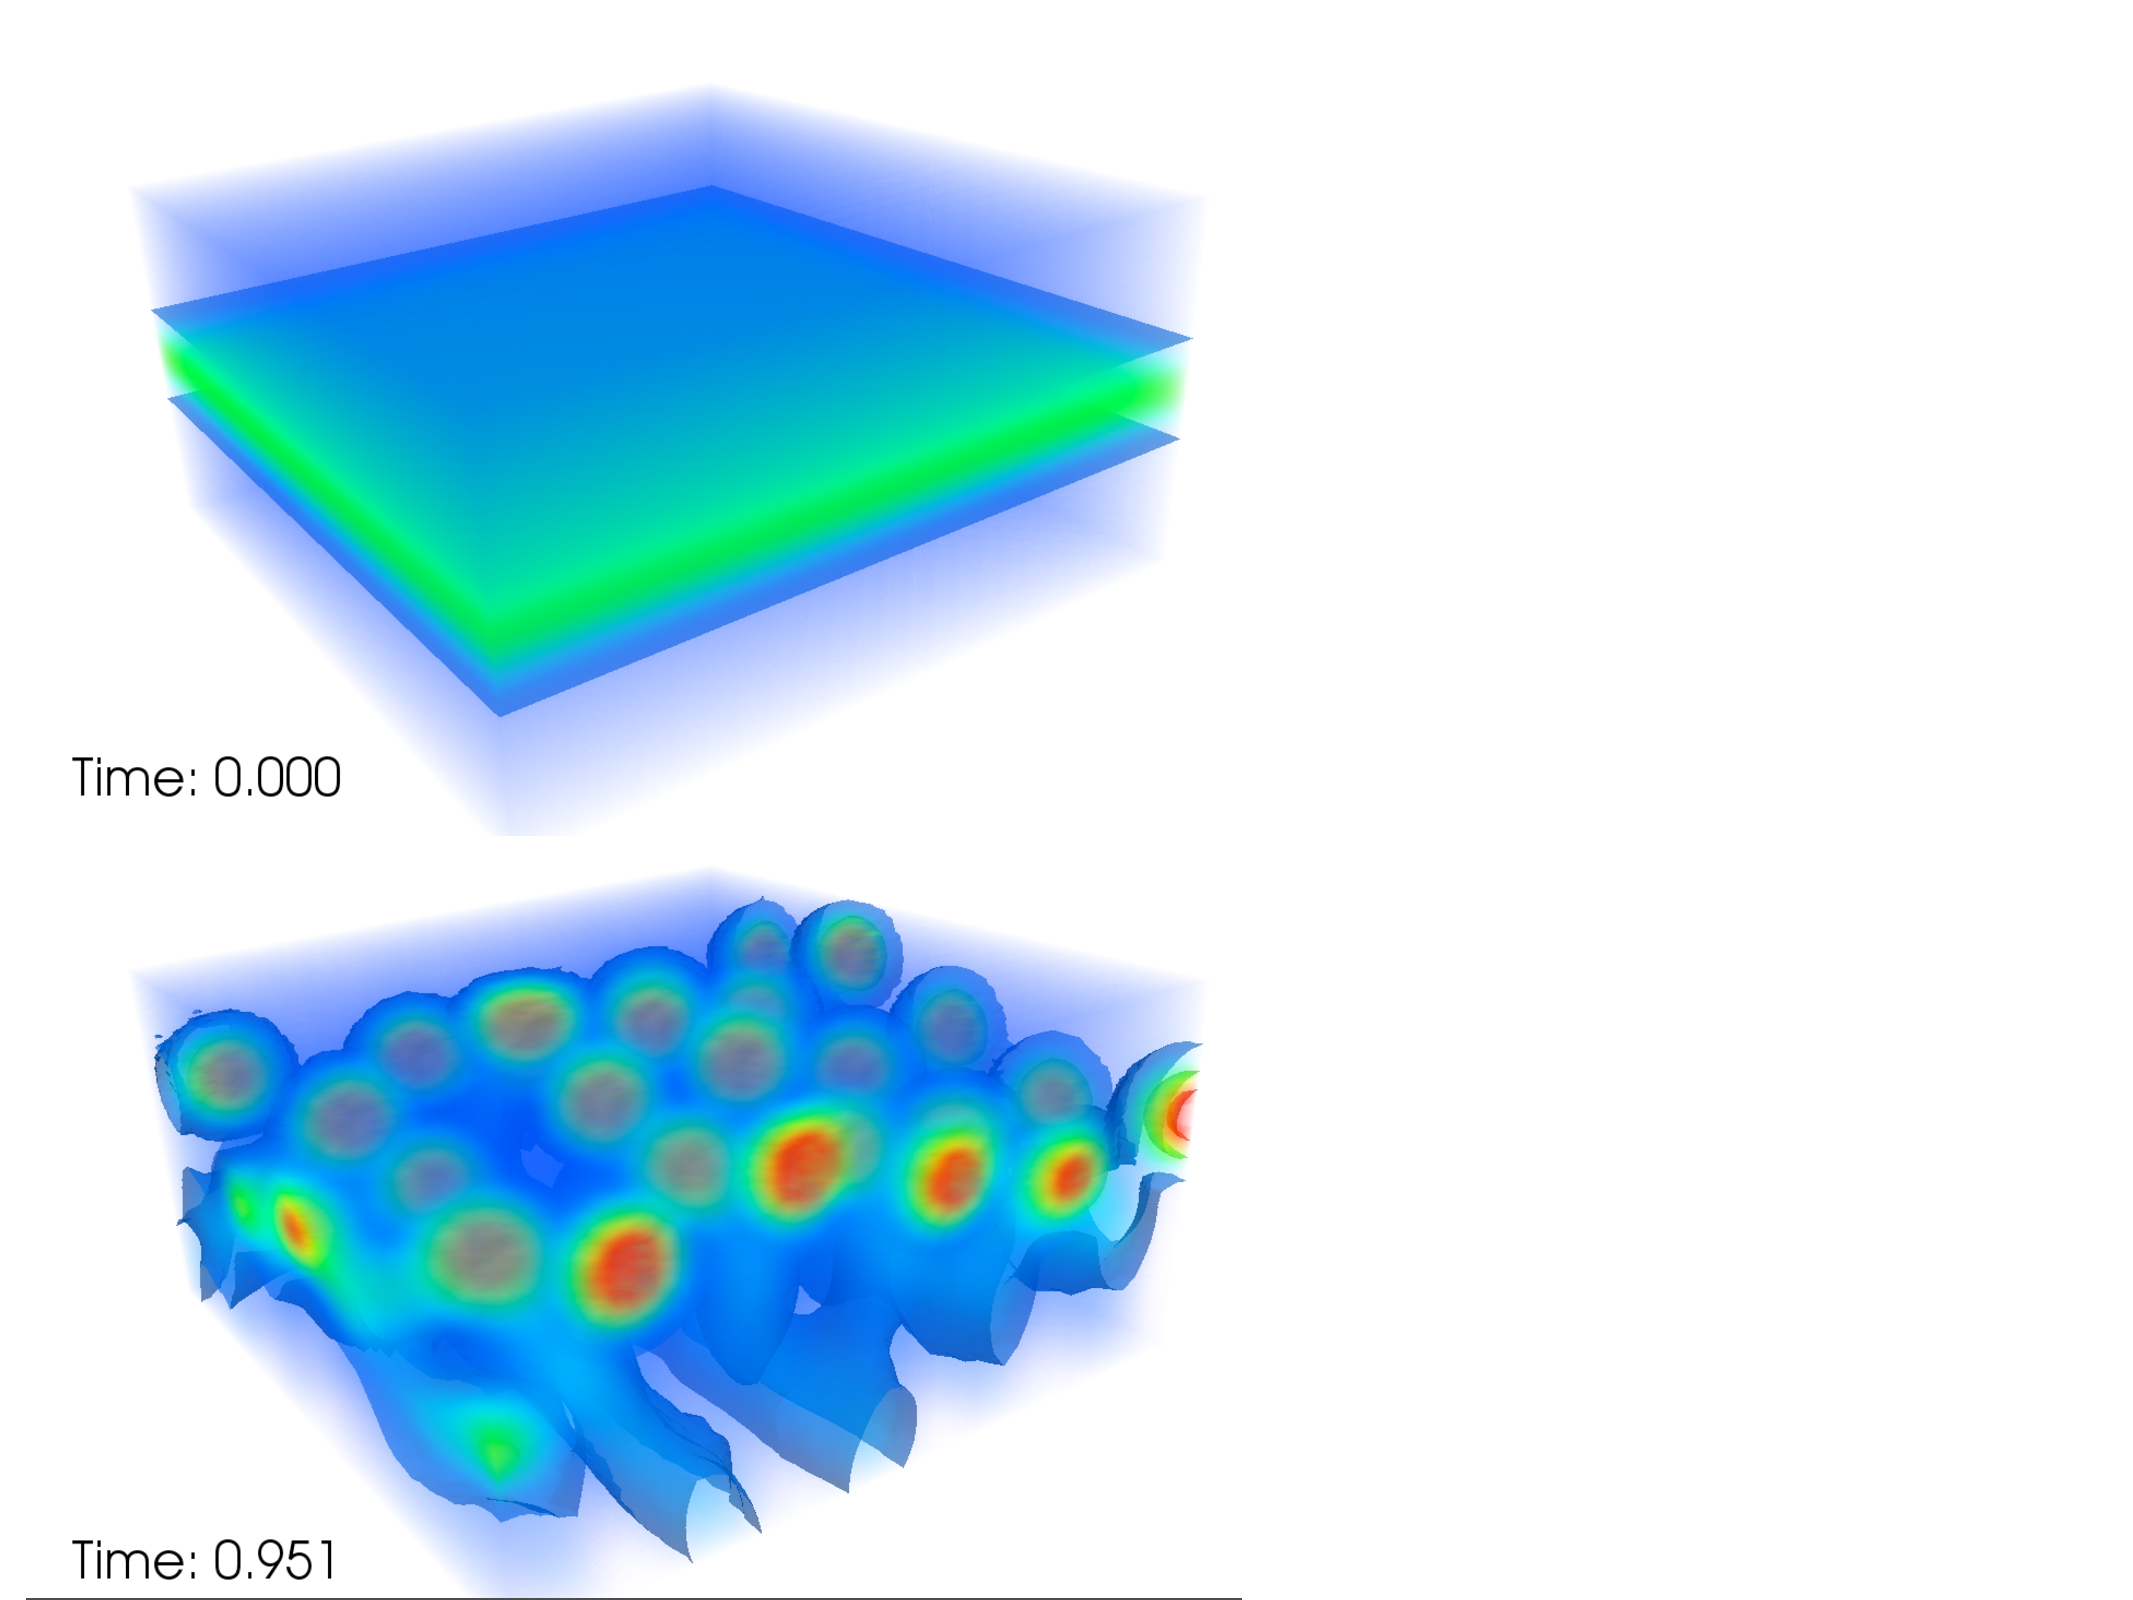
\includegraphics[width=.5\textwidth,clip=true]{figures/1dto3dwaves}
  \caption{Instability of 1D solitary wave to spherical 3D solitary waves.}
  \label{fig:1dto3dwaves}
\end{figure}

\begin{figure}[hb]
  \centering
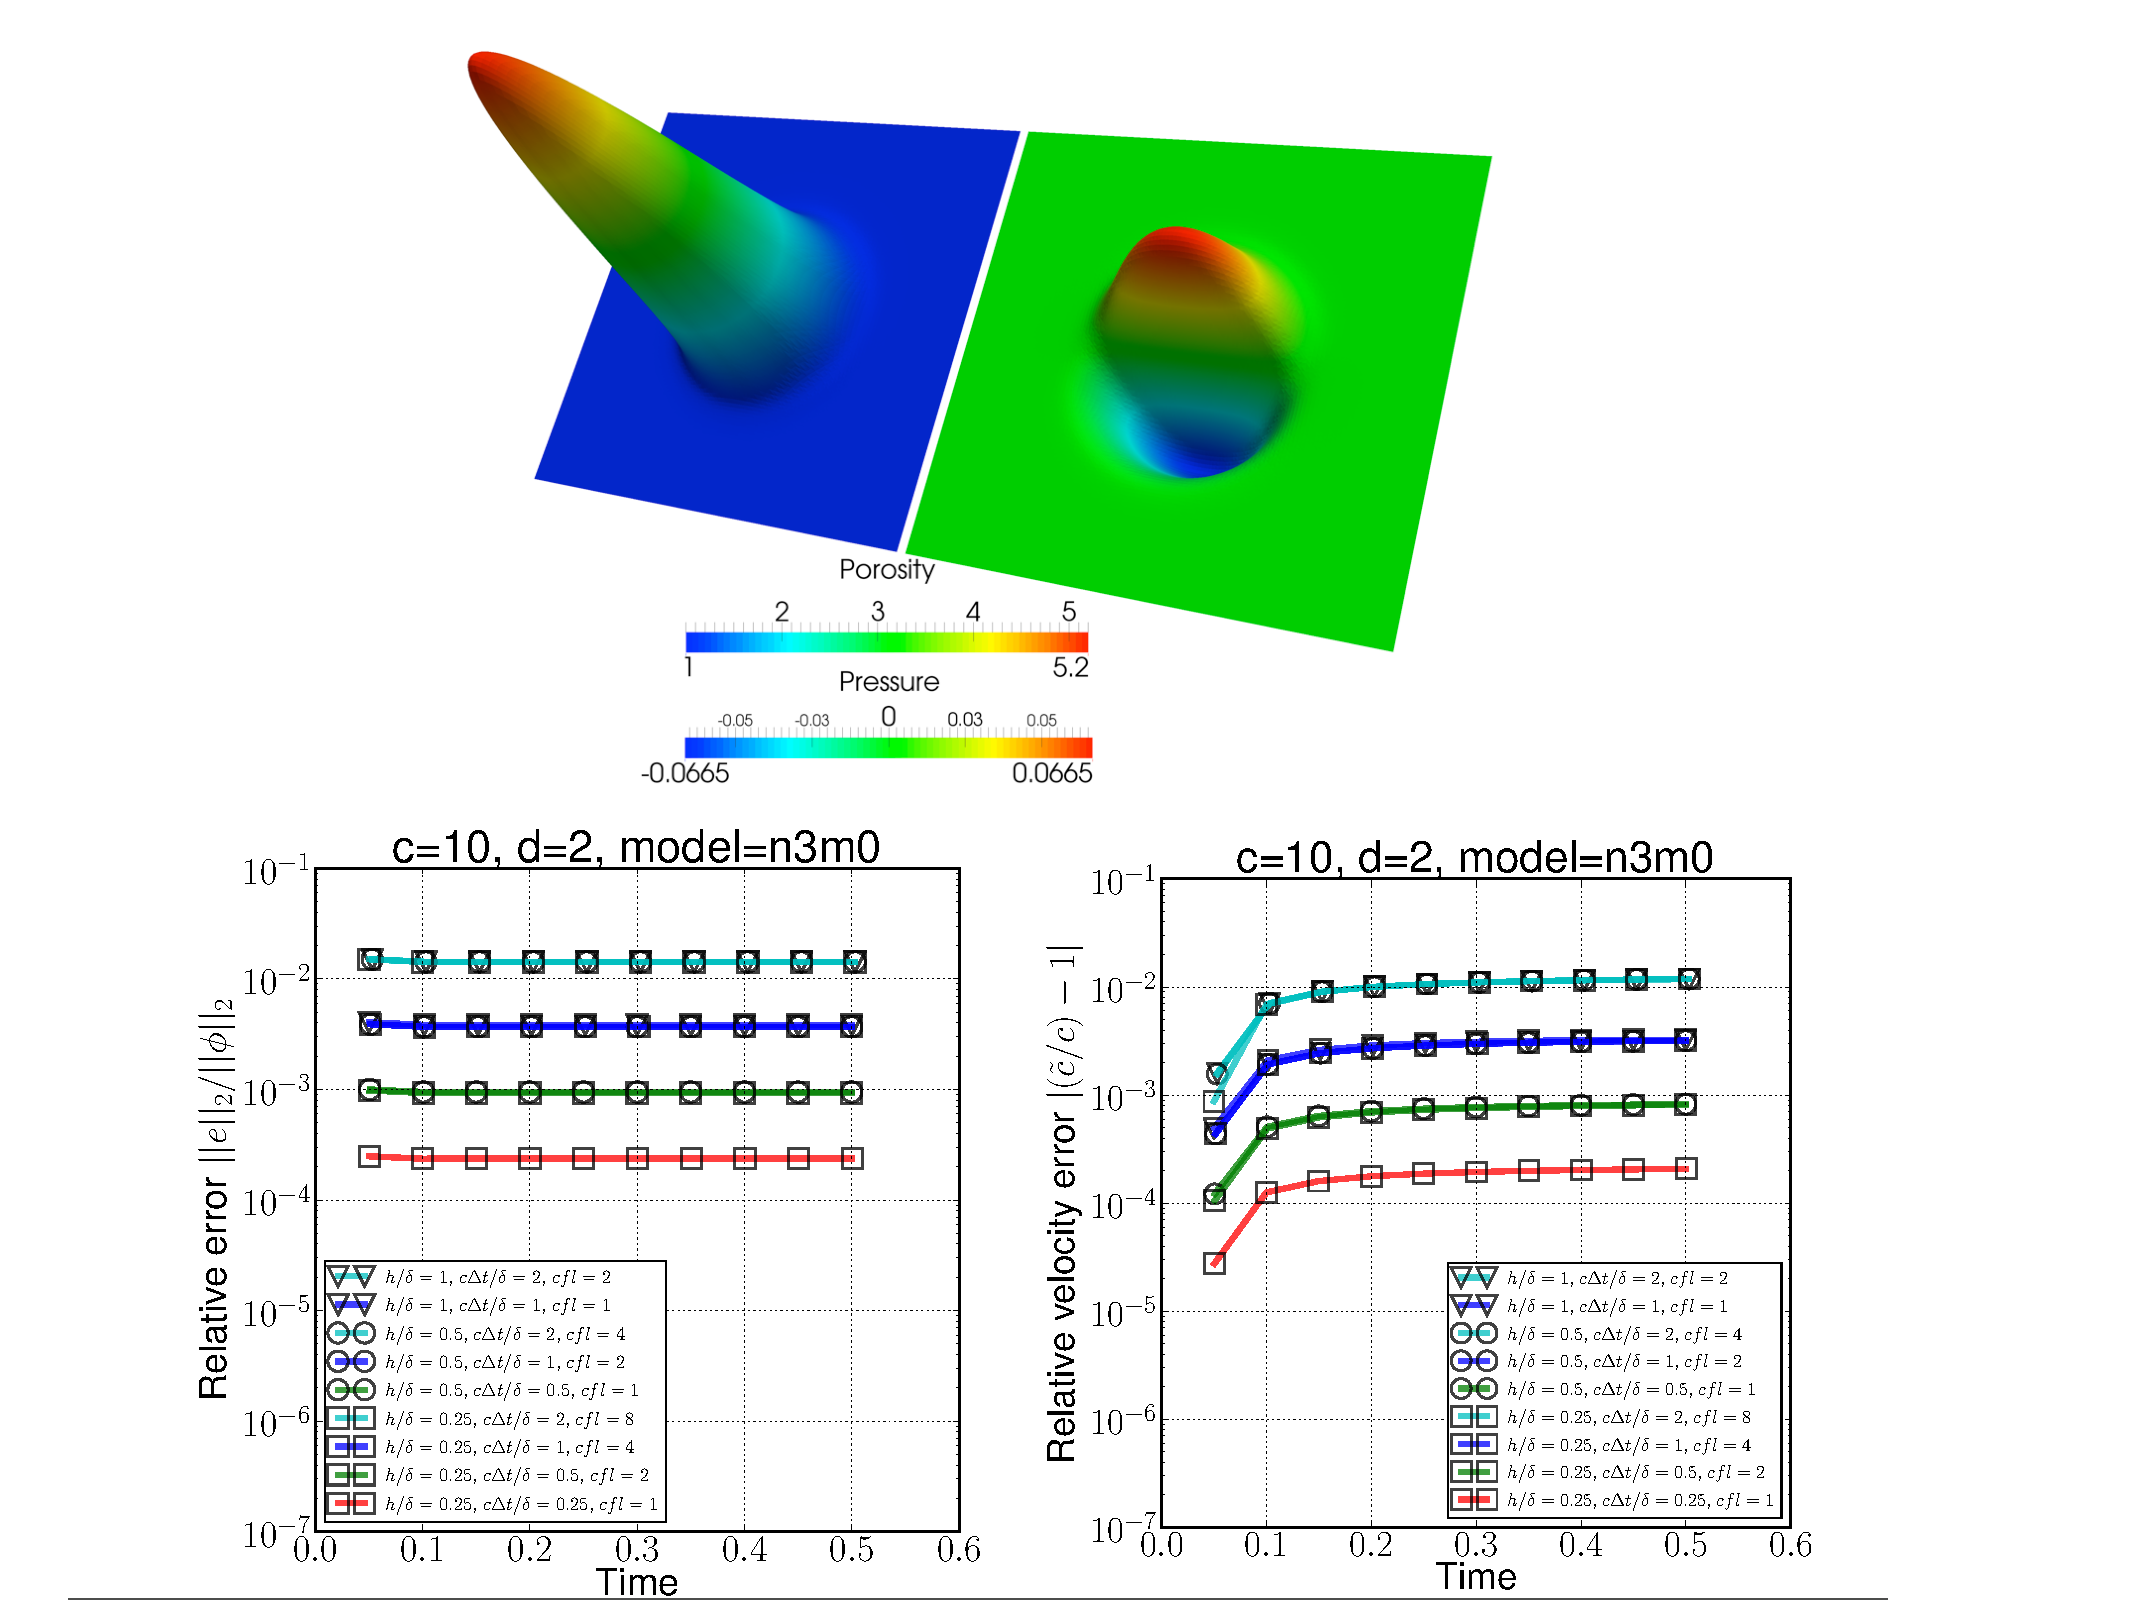
\includegraphics[width=.7\textwidth,clip=true]{figures/simpson_benchmark}
  \caption{Example magmatic solitary wave benchmarks from
    \cite{simpson_solitary_2011}. Top figure shows porosity and
    pressure fields for a 2D porosity wave with speed $c=10$,
    permeability exponent $n=3$, and bulk-viscosity exponent $m=0$.  These waves should propagate at constant porosity $c$
    without changing form and provides a fully non-linear benchmark
    problem. Lower figures show shape and velocity errors as a
    function of time. This benchmark solves the problem in a frame
    moving with the solitary waves using a semi-Lagrangian advection
    scheme in \TF{}. Additional results for other amplitude waves in
    2D and 3D, and other advection schemes are in Tables \ref{tab:simpson2d}--\ref{tab:simpson3d}.  }
  \label{fig:simpson_benchmarks}
\end{figure}

\begin{table*}[th!]
\caption{2D Solitary Wave Benchmarks
    \citep{simpson_solitary_2011}, phase and velocity errors as a
  function of grid-spacing and time step for waves with
  different parameters and background advection schemes, domain height
$h=64\delta$ compaction lengths.}
\begin{center}
  \begin{tabular}{ll}
\fbox{\begin{minipage}[c]{0.075\textwidth}\begin{sideways}\parbox{3.25cm}{\begin{center}$c=10,n=3,m=0$,\\semi-Lagrangian\end{center}}\end{sideways}\end{minipage}} 
&
\fbox{\begin{minipage}[c]{0.575\textwidth}\begin{tabular}{cccc}
     $N$ & $c\Delta t/\delta$  & $||\epsilon_{\phi}||$ & $\epsilon_{c}$  \\
32$\times$32 & 2.00 & 1.427786e-02 & 1.182138e-02  \\
32$\times$32 & 1.00 & 3.819159e-03 & 3.255477e-03  \\
32$\times$32 & 0.50 & 1.634865e-03 & 8.485232e-04  \\
32$\times$32 & 0.25 & 2.202831e-03 & 3.357135e-04  \\
64$\times$64 & 2.00 & 1.424202e-02 & 1.188175e-02  \\
64$\times$64 & 1.00 & 3.690917e-03 & 3.187174e-03  \\
64$\times$64 & 0.50 & 9.481209e-04 & 8.235713e-04  \\
64$\times$64 & 0.25 & 4.243532e-04 & 1.921914e-04  \\
128$\times$128 & 2.00 & 1.424087e-02 & 1.188190e-02  \\
128$\times$128 & 1.00 & 3.686779e-03 & 3.194658e-03  \\
128$\times$128 & 0.50 & 9.306871e-04 & 8.119311e-04  \\
128$\times$128 & 0.25 & 2.365556e-04 & 2.073026e-04  \\
\end{tabular}
\end{minipage}} \\
\\
\fbox{\begin{minipage}[c]{0.075\textwidth}\begin{sideways}\parbox{3.25cm}{\begin{center}$c=10,n=3,m=0$,\\CG\end{center}}\end{sideways}\end{minipage}} 
&
\fbox{\begin{minipage}[c]{0.575\textwidth}\begin{tabular}{cccc}
     $N$ & $c\Delta t/\delta$  & $||\epsilon_{\phi}||$ & $\epsilon_{c}$  \\
32$\times$32 & 2.00 & 1.427786e-02 & 1.182138e-02  \\
32$\times$32 & 1.00 & 3.819159e-03 & 3.255477e-03  \\
32$\times$32 & 0.50 & 1.634865e-03 & 8.485232e-04  \\
32$\times$32 & 0.25 & 2.202831e-03 & 3.357135e-04  \\
64$\times$64 & 2.00 & 1.424202e-02 & 1.188175e-02  \\
64$\times$64 & 1.00 & 3.690917e-03 & 3.187174e-03  \\
64$\times$64 & 0.50 & 9.481209e-04 & 8.235713e-04  \\
64$\times$64 & 0.25 & 4.243532e-04 & 1.921914e-04  \\
128$\times$128 & 2.00 & 1.424087e-02 & 1.188190e-02  \\
128$\times$128 & 1.00 & 3.686779e-03 & 3.194658e-03  \\
128$\times$128 & 0.50 & 9.306871e-04 & 8.119311e-04  \\
128$\times$128 & 0.25 & 2.365556e-04 & 2.073026e-04  \\
\end{tabular}
\end{minipage}} \\
\\
\fbox{\begin{minipage}[c]{0.075\textwidth}\begin{sideways}\parbox{3.25cm}{\begin{center}$c=4,n=2,m=1$,\\semi-Lagrangian\end{center}}\end{sideways}\end{minipage}} 
&
\fbox{\begin{minipage}[c]{0.575\textwidth}\begin{tabular}{cccc}
     $N$ & $c\Delta t/\delta$  & $||\epsilon_{\phi}||$ & $\epsilon_{c}$  \\
32$\times$32 & 2.00 & 1.427786e-02 & 1.182138e-02  \\
32$\times$32 & 1.00 & 3.819159e-03 & 3.255477e-03  \\
32$\times$32 & 0.50 & 1.634865e-03 & 8.485232e-04  \\
32$\times$32 & 0.25 & 2.202831e-03 & 3.357135e-04  \\
64$\times$64 & 2.00 & 1.424202e-02 & 1.188175e-02  \\
64$\times$64 & 1.00 & 3.690917e-03 & 3.187174e-03  \\
64$\times$64 & 0.50 & 9.481209e-04 & 8.235713e-04  \\
64$\times$64 & 0.25 & 4.243532e-04 & 1.921914e-04  \\
128$\times$128 & 2.00 & 1.424087e-02 & 1.188190e-02  \\
128$\times$128 & 1.00 & 3.686779e-03 & 3.194658e-03  \\
128$\times$128 & 0.50 & 9.306871e-04 & 8.119311e-04  \\
128$\times$128 & 0.25 & 2.365556e-04 & 2.073026e-04  \\
\end{tabular}
\end{minipage}} \\
\\
\fbox{\begin{minipage}[c]{0.075\textwidth}\begin{sideways}\parbox{3.25cm}{\begin{center}$c=4,n=2,m=1$,\\CG\end{center}}\end{sideways}\end{minipage}} 
&
\fbox{\begin{minipage}[c]{0.575\textwidth}\begin{tabular}{cccc}
     $N$ & $c\Delta t/\delta$  & $||\epsilon_{\phi}||$ & $\epsilon_{c}$  \\
32$\times$32 & 2.00 & 1.427786e-02 & 1.182138e-02  \\
32$\times$32 & 1.00 & 3.819159e-03 & 3.255477e-03  \\
32$\times$32 & 0.50 & 1.634865e-03 & 8.485232e-04  \\
32$\times$32 & 0.25 & 2.202831e-03 & 3.357135e-04  \\
64$\times$64 & 2.00 & 1.424202e-02 & 1.188175e-02  \\
64$\times$64 & 1.00 & 3.690917e-03 & 3.187174e-03  \\
64$\times$64 & 0.50 & 9.481209e-04 & 8.235713e-04  \\
64$\times$64 & 0.25 & 4.243532e-04 & 1.921914e-04  \\
128$\times$128 & 2.00 & 1.424087e-02 & 1.188190e-02  \\
128$\times$128 & 1.00 & 3.686779e-03 & 3.194658e-03  \\
128$\times$128 & 0.50 & 9.306871e-04 & 8.119311e-04  \\
128$\times$128 & 0.25 & 2.365556e-04 & 2.073026e-04  \\
\end{tabular}
\end{minipage}}
  \end{tabular}
\end{center}
\label{tab:simpson2d}
\end{table*}

\begin{table*}[th!]
\caption{3D Solitary Wave Benchmarks
    \citep{simpson_solitary_2011}, phase and velocity errors as a
  function of grid-spacing and time step, CG advection, $c=5$, $n=3$,
  $m=0$ waves}
\begin{center}
  \begin{tabular}{ll}
\fbox{\begin{minipage}[c]{0.075\textwidth}\begin{sideways}\parbox{3.25cm}{\begin{center}$h/\delta=64$\end{center}}\end{sideways}\end{minipage}} 
&
\fbox{\begin{minipage}[c]{0.575\textwidth}\begin{tabular}{cccc}
     $N$ & $c\Delta t/\delta$  & $||\epsilon_{\phi}||$ & $\epsilon_{c}$  \\
32$\times$32 & 2.00 & 1.427786e-02 & 1.182138e-02  \\
32$\times$32 & 1.00 & 3.819159e-03 & 3.255477e-03  \\
32$\times$32 & 0.50 & 1.634865e-03 & 8.485232e-04  \\
32$\times$32 & 0.25 & 2.202831e-03 & 3.357135e-04  \\
64$\times$64 & 2.00 & 1.424202e-02 & 1.188175e-02  \\
64$\times$64 & 1.00 & 3.690917e-03 & 3.187174e-03  \\
64$\times$64 & 0.50 & 9.481209e-04 & 8.235713e-04  \\
64$\times$64 & 0.25 & 4.243532e-04 & 1.921914e-04  \\
128$\times$128 & 2.00 & 1.424087e-02 & 1.188190e-02  \\
128$\times$128 & 1.00 & 3.686779e-03 & 3.194658e-03  \\
128$\times$128 & 0.50 & 9.306871e-04 & 8.119311e-04  \\
128$\times$128 & 0.25 & 2.365556e-04 & 2.073026e-04  \\
\end{tabular}
\end{minipage}} \\
\\
\fbox{\begin{minipage}[c]{0.075\textwidth}\begin{sideways}\parbox{3.25cm}{\begin{center}$h/\delta=32$\\(higher resolution)\end{center}}\end{sideways}\end{minipage}} 
&
\fbox{\begin{minipage}[c]{0.575\textwidth}\begin{tabular}{cccc}
     $N$ & $c\Delta t/\delta$  & $||\epsilon_{\phi}||$ & $\epsilon_{c}$  \\
32$\times$32 & 2.00 & 1.427786e-02 & 1.182138e-02  \\
32$\times$32 & 1.00 & 3.819159e-03 & 3.255477e-03  \\
32$\times$32 & 0.50 & 1.634865e-03 & 8.485232e-04  \\
32$\times$32 & 0.25 & 2.202831e-03 & 3.357135e-04  \\
64$\times$64 & 2.00 & 1.424202e-02 & 1.188175e-02  \\
64$\times$64 & 1.00 & 3.690917e-03 & 3.187174e-03  \\
64$\times$64 & 0.50 & 9.481209e-04 & 8.235713e-04  \\
64$\times$64 & 0.25 & 4.243532e-04 & 1.921914e-04  \\
128$\times$128 & 2.00 & 1.424087e-02 & 1.188190e-02  \\
128$\times$128 & 1.00 & 3.686779e-03 & 3.194658e-03  \\
128$\times$128 & 0.50 & 9.306871e-04 & 8.119311e-04  \\
128$\times$128 & 0.25 & 2.365556e-04 & 2.073026e-04  \\
\end{tabular}
\end{minipage}}
  \end{tabular}
\end{center}
\label{tab:simpson3d}
\end{table*}



\bibliographystyle{plainnat}
\bibliography{tfbenchmarksrefs.bib}
\end{document}


